\section{Results}
\label{sec:results}

We report the results in two parts, one per experiment of Section~\ref{sec:evaluation_methodology}: the planner-stage latency with deconfliction disabled (RQ1), and the runs with conflict checking enabled (RQ2 and RQ3). Appendix~\ref{sec:blan_wohl_trajectory} shows one example request from start to end---route, waypoints, altitude and speed---for readers who want to see what the pipeline produces before looking at the numbers.

\subsection{Planner-Stage Latency Decomposition and Route-Length Dependence}
\label{sec:planner_scalability}

This experiment tests the Planning Service alone, without the Deconfliction Service. It is a sequential baseline over one fixed batch of requests and shows how the latency depends on path length on one fixed network; it does not test concurrent load or larger networks. \paPairs{} random origin--destination pairs were processed one after another, each pair \paReps{} times after five warmup requests, which gives \paObs{} timing observations over \paPairs{} different routes. All requests used the Hamburg corridor graph and the fixed \SI{200}{m} MSL cruise layer. All requests succeeded, so no failed cases were removed. As explained in Section~\ref{sec:evaluation_methodology}, the runtime distributions below use all \paObs{} observations, and all regressions, confidence intervals and correlations use the \paPairs{} per-pair means.

Table~\ref{tab:planner_scalability_runtime} shows the runtime of the planner stages. We call the sum of A* search, waypoint synthesis, and CFMS invocation and dense trajectory generation the \emph{planner-stage subtotal}. Its mean is \SI{\paPlannerMean}{ms}, its \(p_{90}\) is \SI{\paPlannerPninety}{ms}, and its maximum is \SI{\paPlannerMax}{ms} over the \paObs{} observations. These latencies are consistent with interactive use in the evaluated local setup; they do not characterize operation under distributed or concurrent load. Most of this time is CFMS invocation and dense trajectory generation, with a mean of \SI{\paGenMean}{ms}. Waypoint synthesis and A* search both stay below one millisecond, with maxima of \SI{\paWpMax}{ms} and \SI{\paAstarMax}{ms}.

\begin{table}[H]
  \centering
  \caption{Planner-stage runtime summary over \paObs{} timing observations (\paPairs{} OD pairs \(\times\) \paReps{} repetitions after 5 warmup requests). The sample unit is the individual timing observation, not the route geometry. The median averages the two middle observations; the 90th percentile is an order statistic without interpolation, as defined in Section~\ref{sec:evaluation_methodology}; the maximum is reported instead of a high quantile because \paObs{} observations support at most coarse tail estimates.}
  \label{tab:planner_scalability_runtime}
  \small
  % Table generated by tools/make_planner_stats.py from
  % plots/trajcalc_scalability/planner_scalability.csv. Do not edit by hand.
  \begin{tabular}{lrrrrr}
  \toprule
  Metric & Mean (ms) & Std (ms) & \(p_{50}\) (ms) & \(p_{90}\) (ms) & Max (ms) \\
  \midrule
  Planner-stage subtotal & 47.25 & 18.86 & 44.96 & 73.02 & 111.72 \\
  CFMS invocation + generation & 46.88 & 18.81 & 44.62 & 72.39 & 111.22 \\
  Waypoint synthesis & 0.13 & 0.03 & 0.12 & 0.17 & 0.33 \\
  A* path search & 0.24 & 0.07 & 0.22 & 0.30 & 0.76 \\
  \bottomrule
\end{tabular}

\end{table}

Trajectory generation therefore accounts for almost all of the planning time, while A* and waypoint synthesis are negligible in comparison. Based on the mean values in Table~\ref{tab:planner_scalability_runtime}, it makes up about \paGenShare{}\% of the planner-stage subtotal. Because of this, the subtotal depends on route length in the same way as trajectory generation does.

Figure~\ref{fig:planner_scalability_distance} plots the planner-stage times over path distance, one point per OD pair. The subtotal and the trajectory-generation time both grow clearly with distance (Pearson \(r = \paPlannerDistR{}\) and \(r = \paGenDistR{}\)). A linear regression of the subtotal on path distance gives a slope of \SI{\paPlannerDistSlope}{ms/km} (95\% confidence interval \([\paPlannerDistLo{}, \paPlannerDistHi{}]\), \(R^2 = \paPlannerDistRsq{}\), \(n = \paPairs{}\) OD pairs). Two further regressions support an interpretation of this association. The number of trajectory samples grows almost exactly linearly with distance (\paSamplesDistSlope{} samples per km, 95\% CI \([\paSamplesDistLo{}, \paSamplesDistHi{}]\), \(R^2 = \paSamplesDistRsq{}\)), and the trajectory-generation time grows linearly with the number of samples (\SI{\paGenSamplesSlope}{ms} per sample, 95\% CI \([\paGenSamplesLo{}, \paGenSamplesHi{}]\), \(R^2 = \paGenSamplesRsq{}\)). This is consistent with additional samples contributing to longer runtimes; the experiment does not independently vary sample count at fixed route geometry. Waypoint synthesis (Pearson \(r = \paWpDistR{}\)) and A* search (Pearson \(r = \paAstarDistR{}\)) stay small over the whole distance range. On this network, route search is therefore not the bottleneck.

\begin{figure}[!htbp]
  \centering
  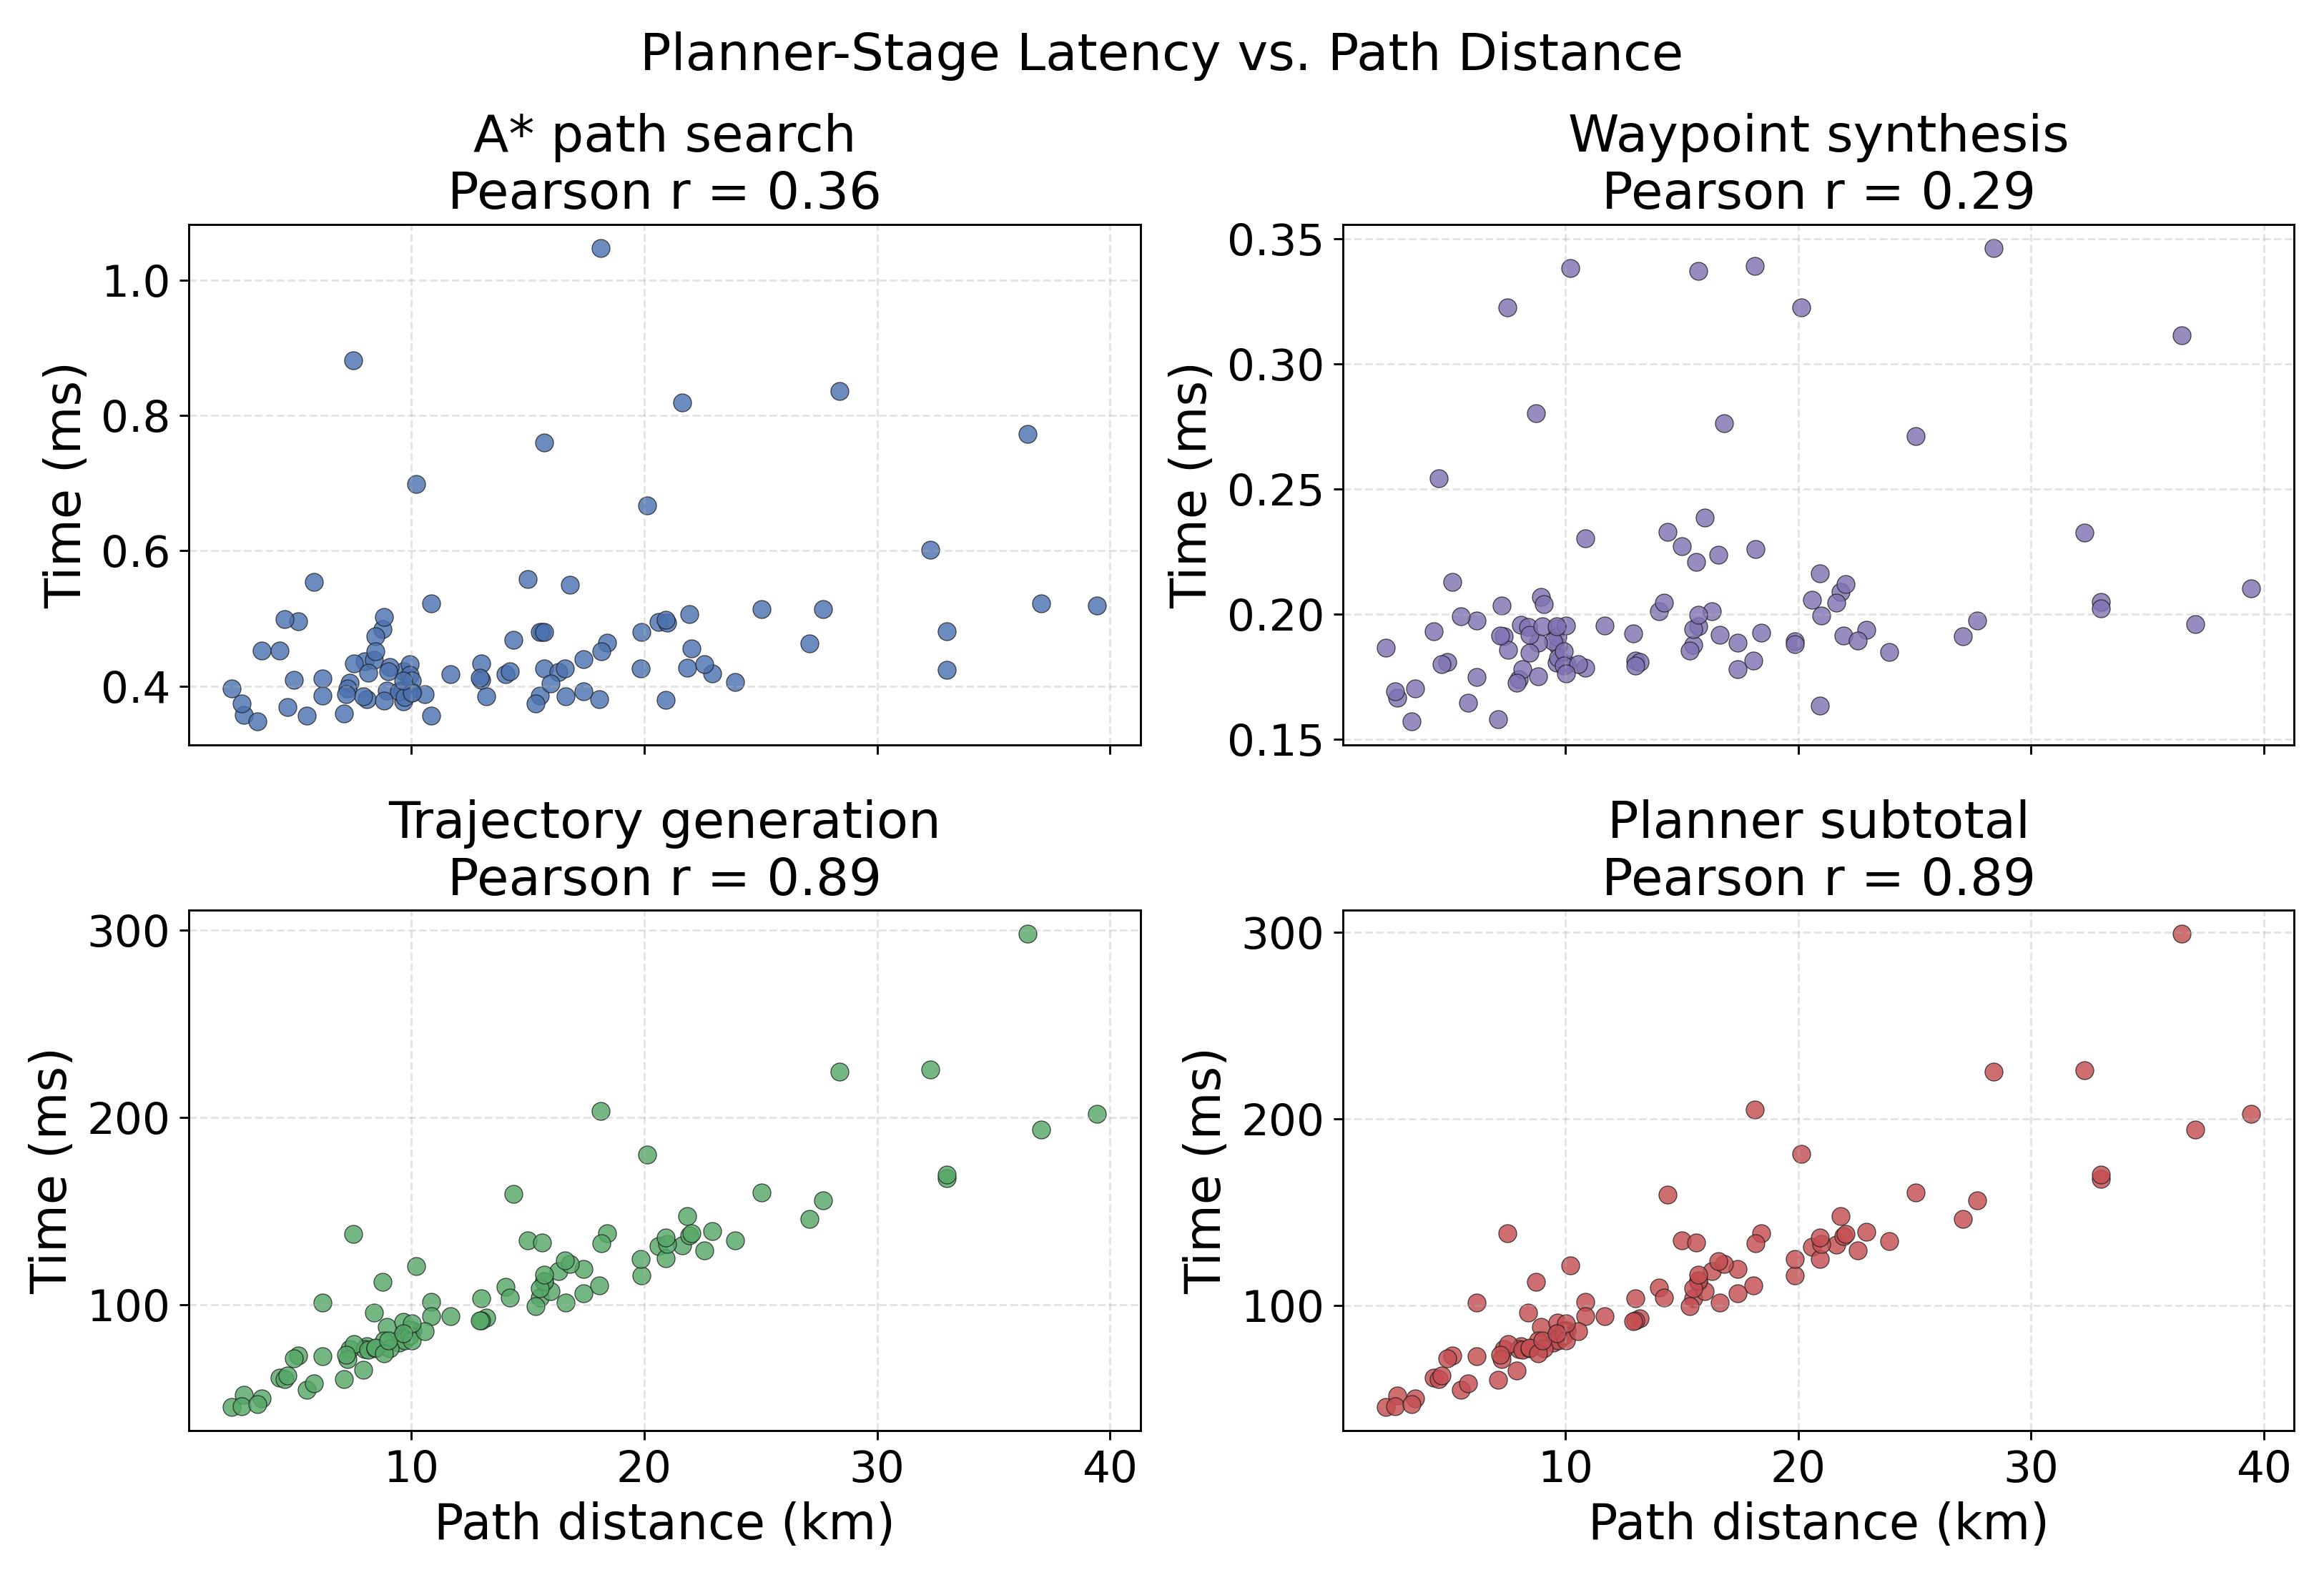
\includegraphics[width=0.90\textwidth]{figures/planner_scalability_stage_times_vs_distance.png}
  \caption{Planner-stage latency as a function of selected path distance. Each point is one of the \paPairs{} origin--destination pairs, plotted at the mean of its \paReps{} repetitions; the dashed line is the ordinary-least-squares fit over those \paPairs{} aggregates. Each panel shows one stage (color-coded) with its Pearson \(r\) annotated in the panel title. The trajectory-generation stage covers CFMS invocation and dense trajectory generation.}
  \label{fig:planner_scalability_distance}
\end{figure}

The boxplots per distance bucket in Figure~\ref{fig:planner_scalability_boxplots} show the same result. Each bucket label gives its number \(n\) of timing observations (\paBucketObsList{} for the \paBucketRanges{} buckets), which are \paBucketPairList{} different OD pairs. The median subtotal and trajectory-generation times both increase from bucket to bucket, but the spread inside a bucket does not grow steadily (standard deviations of \paPlannerBucketStd{}~ms; the small top bucket is narrower than the middle ones). A* stays tightly bounded in all buckets. The histograms in Figure~\ref{fig:planner_scalability_hist} show that the subtotal distribution is essentially the trajectory-generation distribution plus a sub-millisecond part from waypoint synthesis and graph search.

\begin{figure}[H]
  \centering
  \subfloat[Planner-stage subtotal]{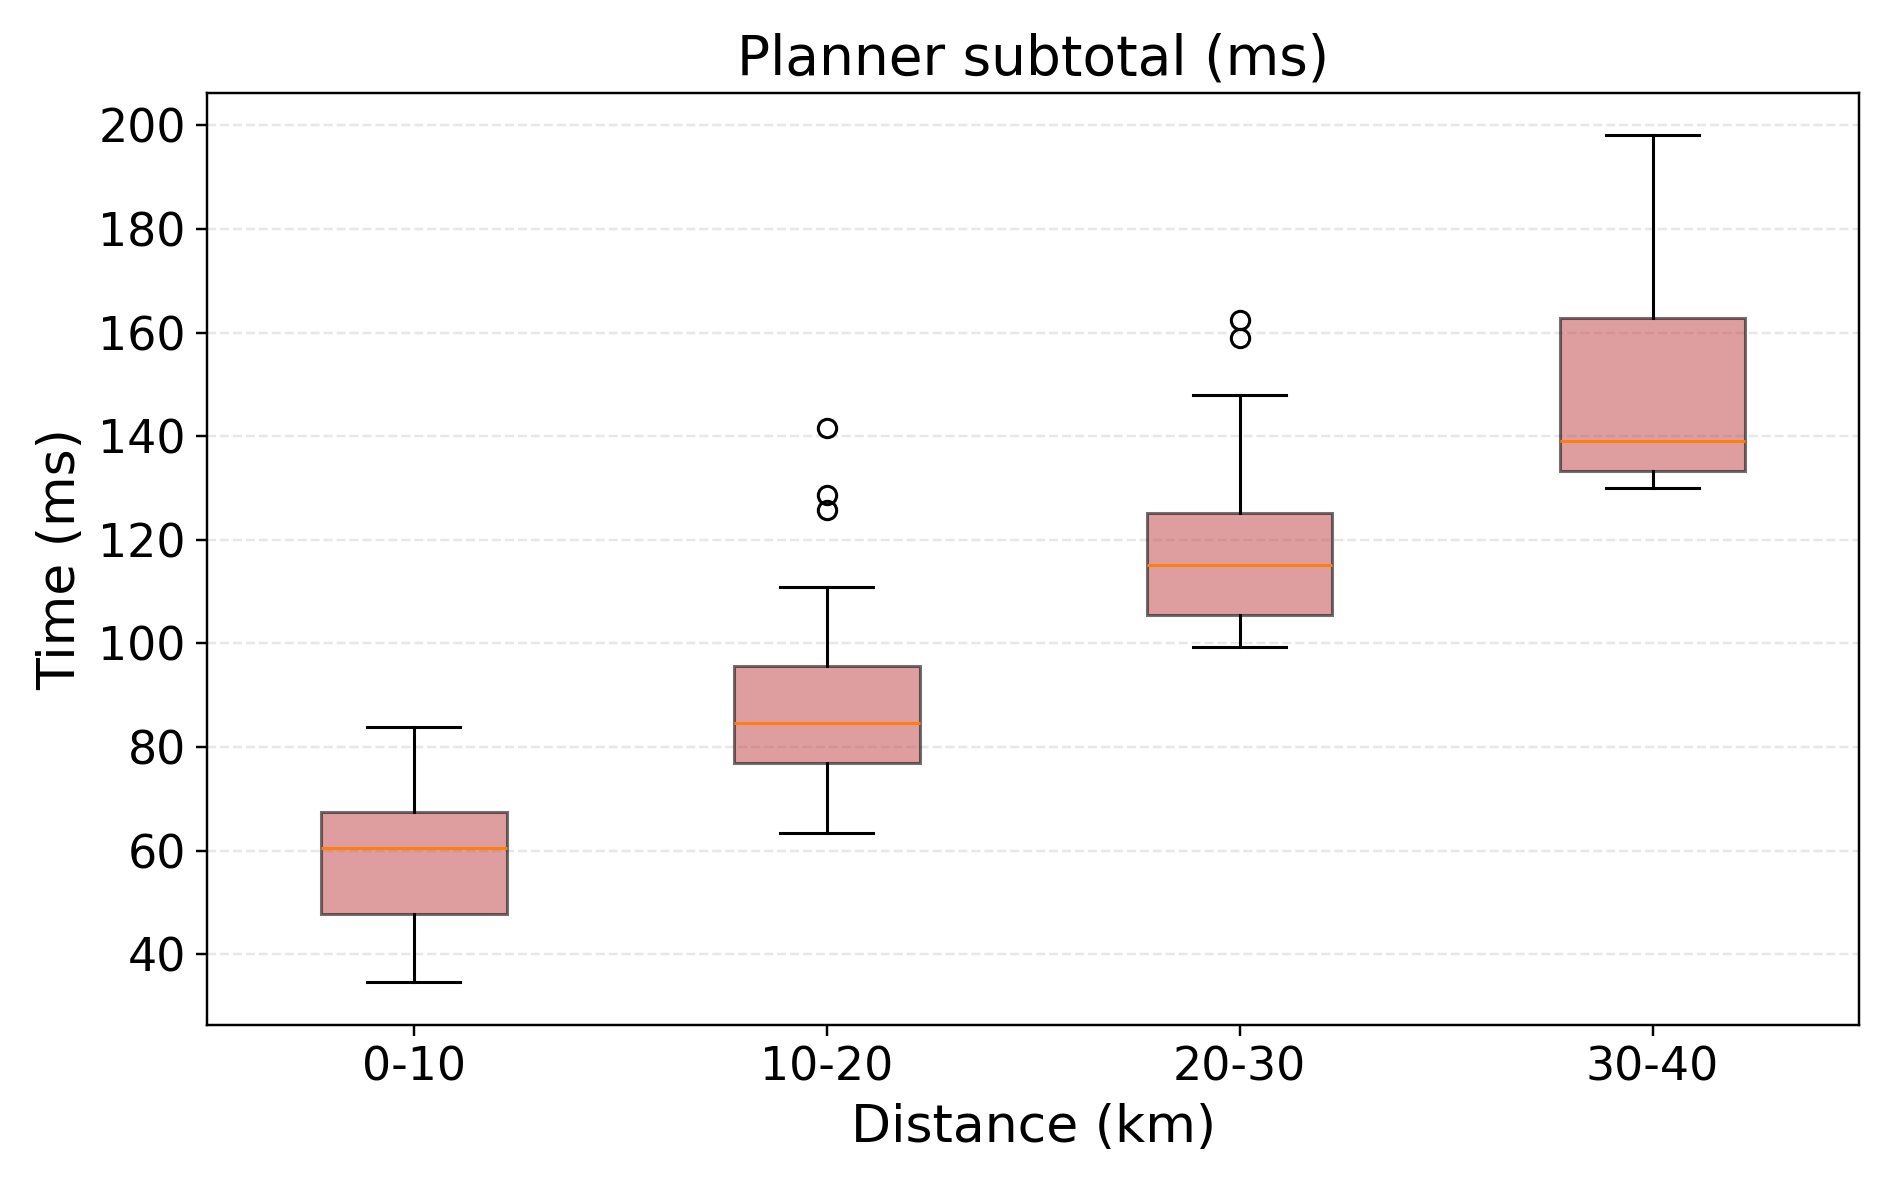
\includegraphics[width=0.46\textwidth]{figures/box_planner_ms_by_distance.png}}
  \hfill
  \subfloat[CFMS invocation + generation]{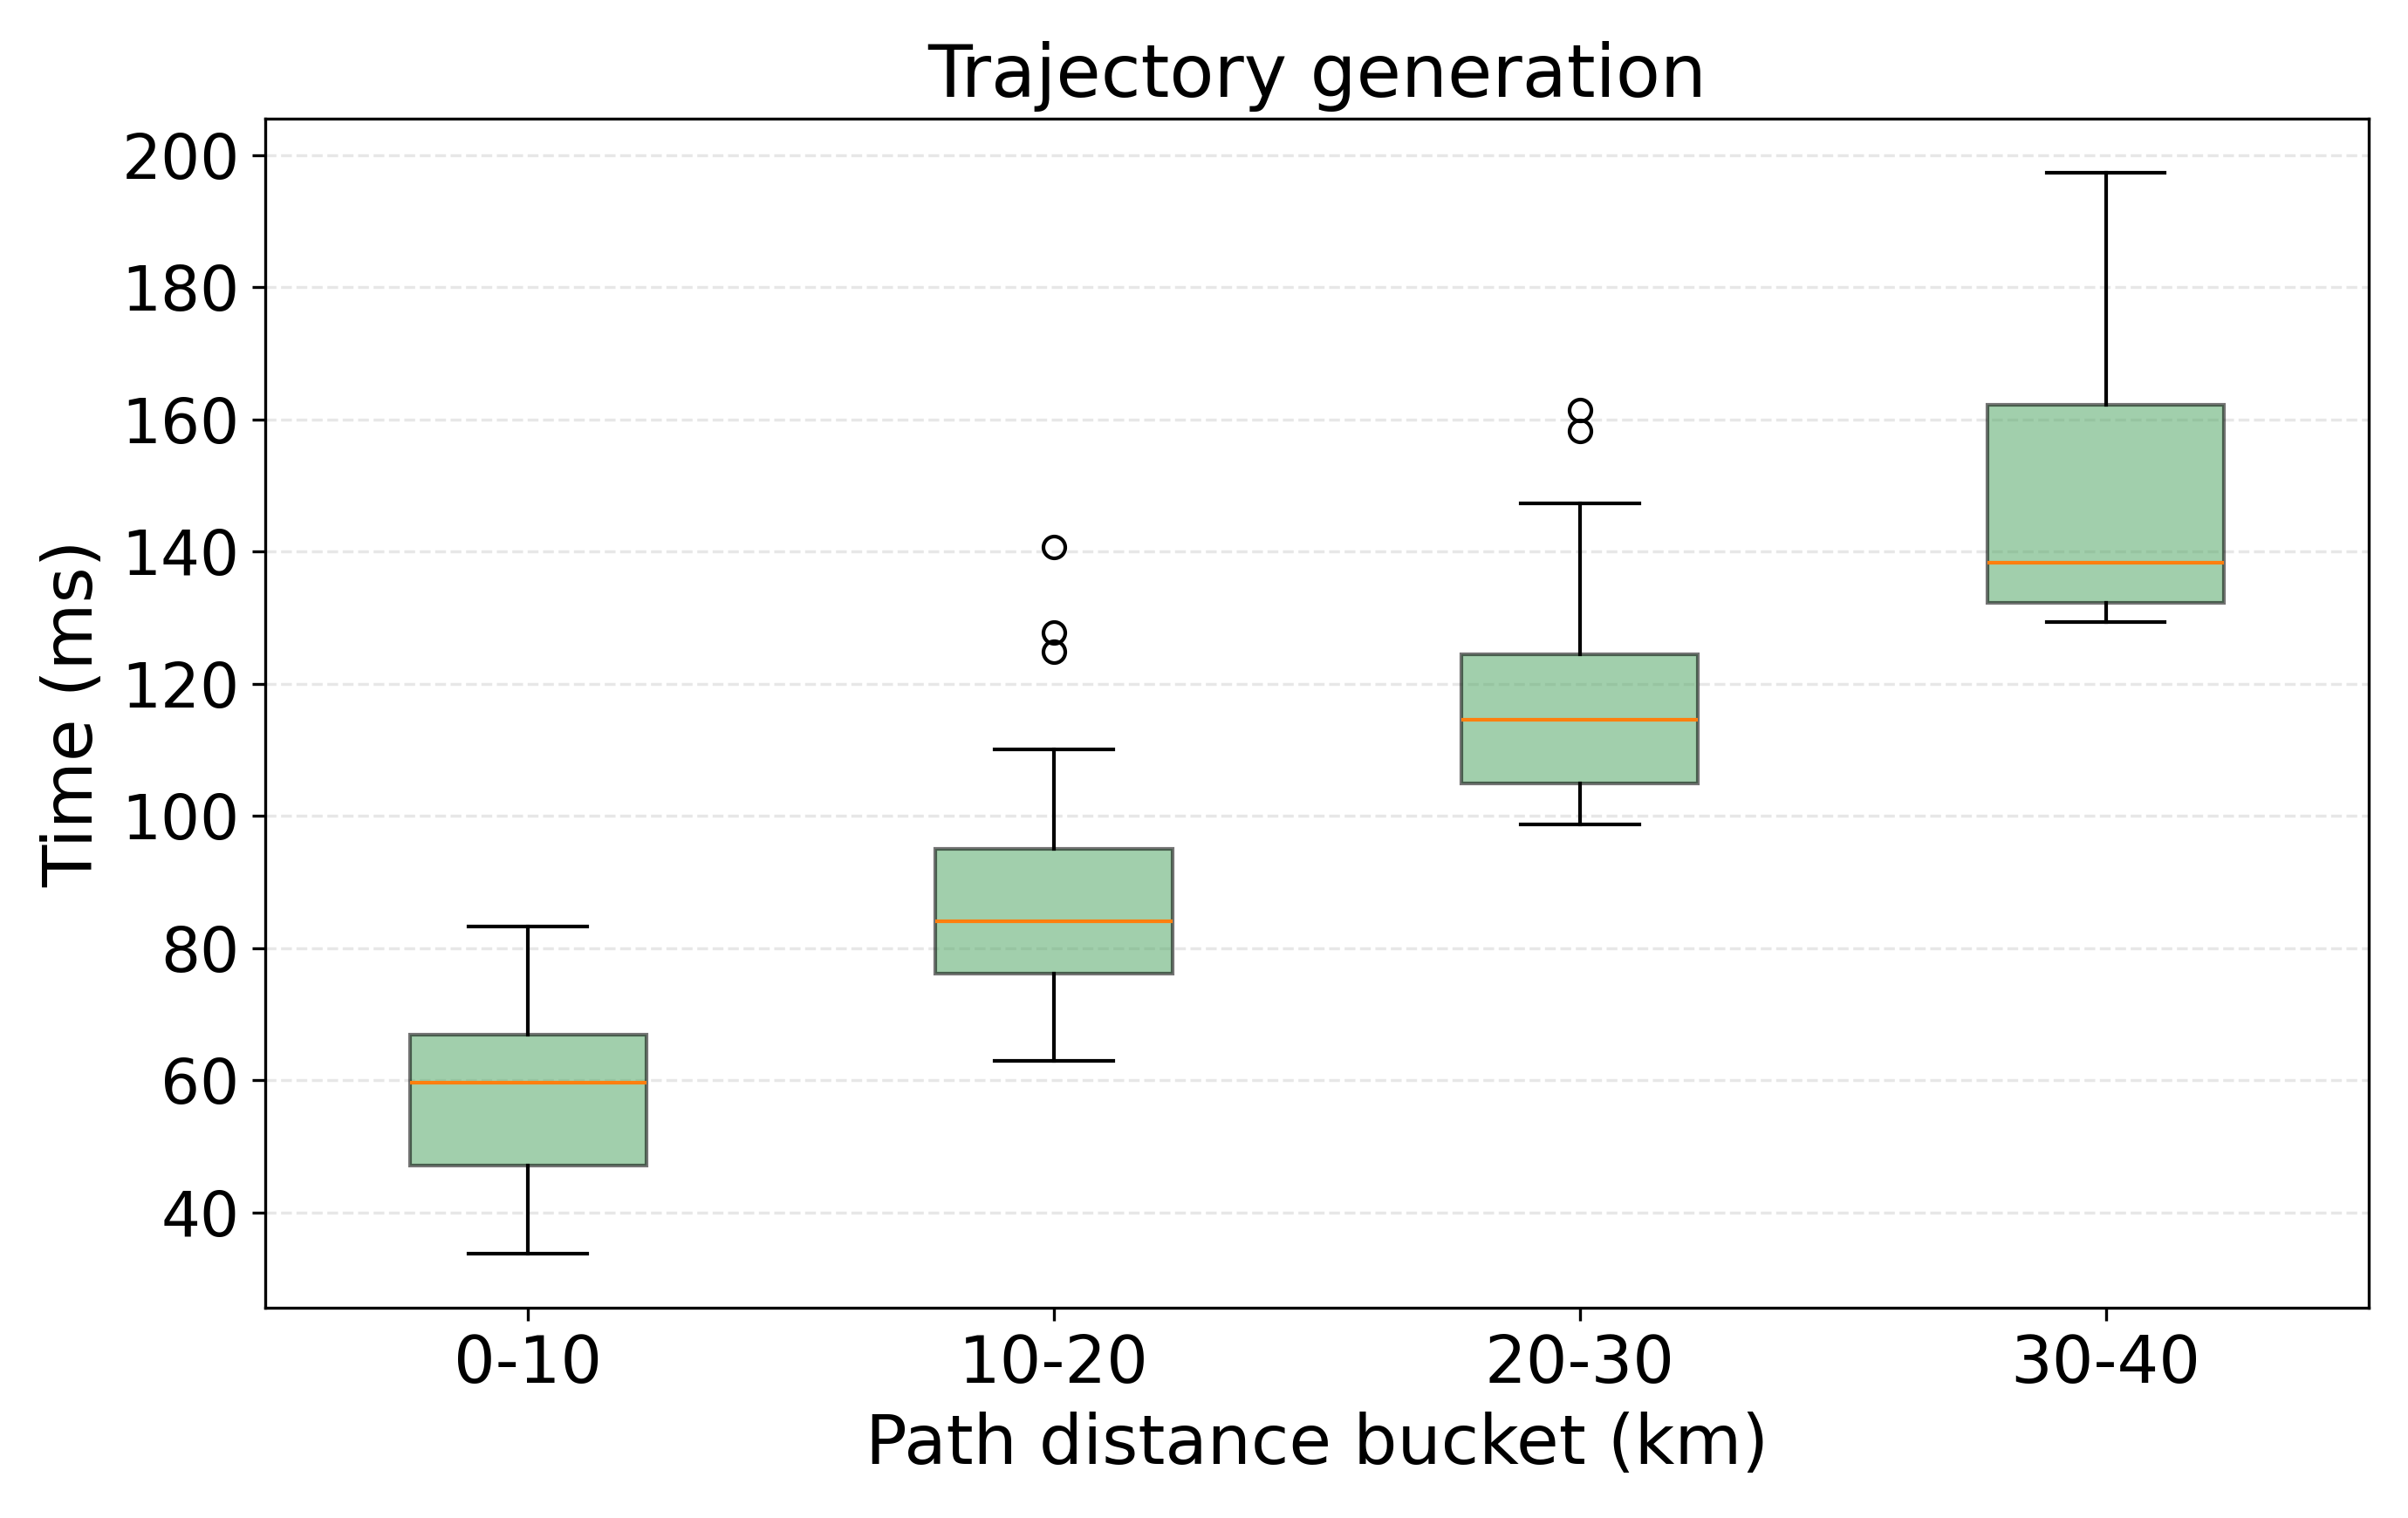
\includegraphics[width=0.46\textwidth]{figures/box_traj_generator_ms_by_distance.png}}
  \vspace{0.2em}
  \subfloat[A* path search]{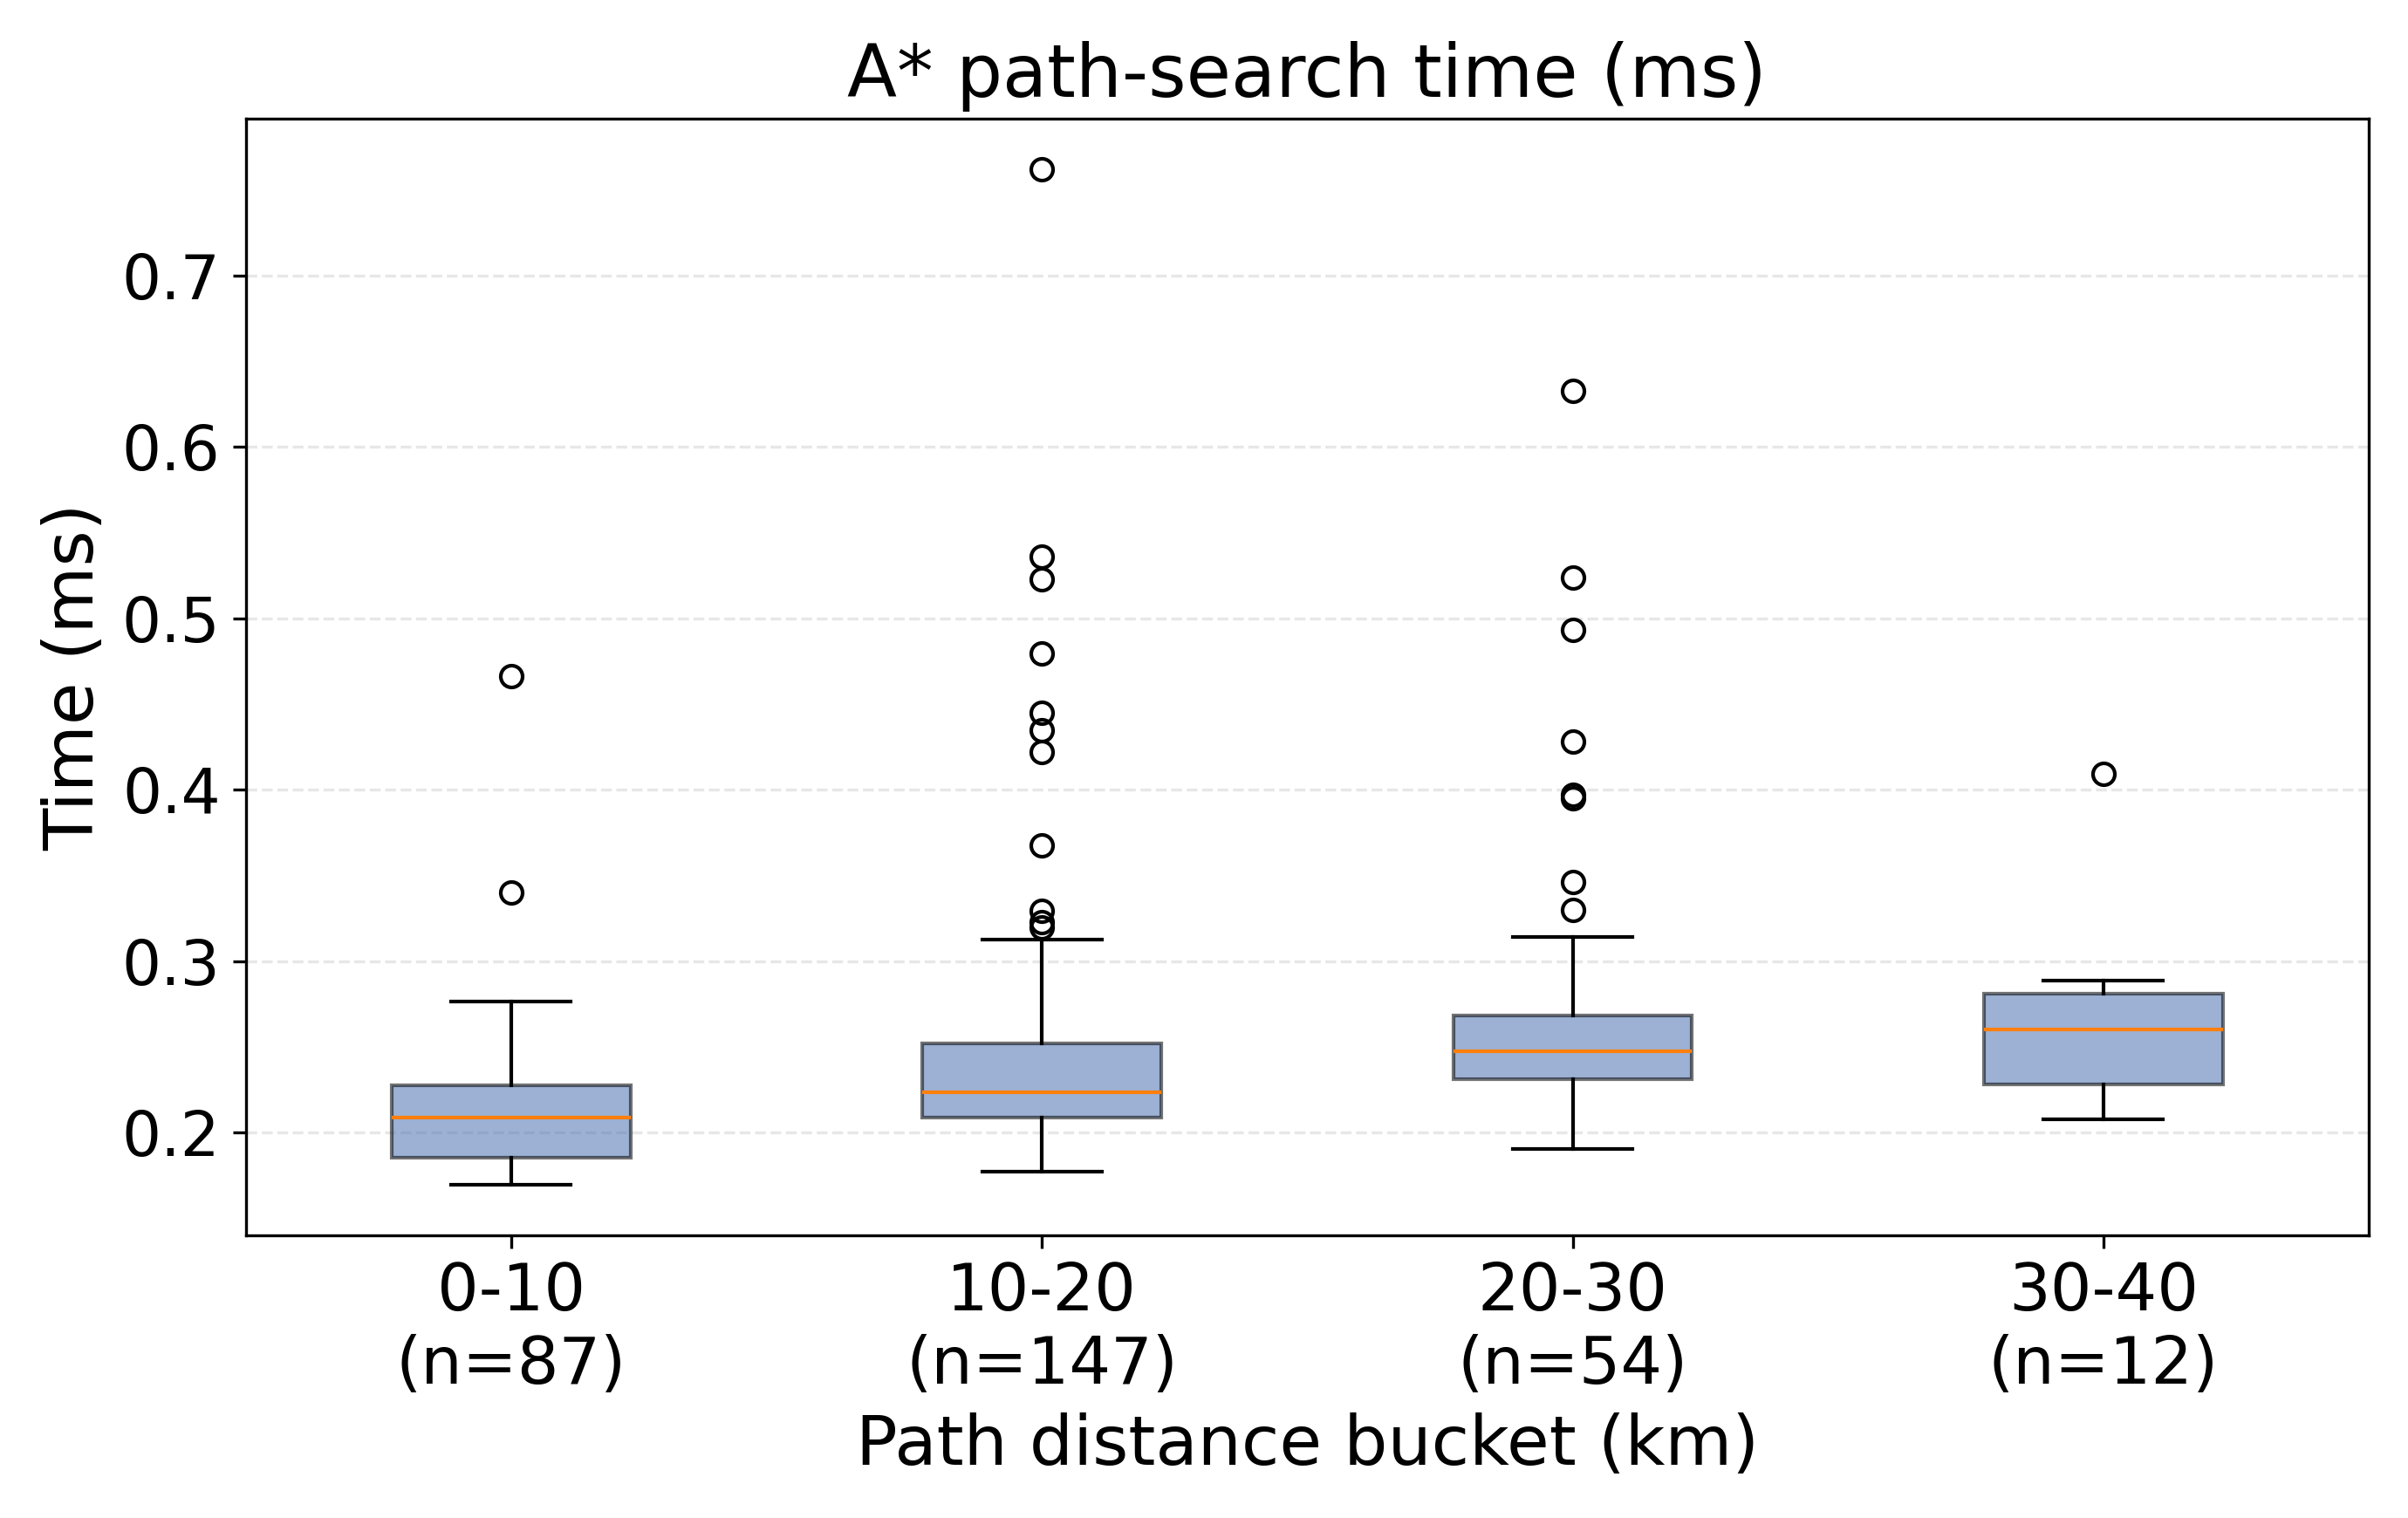
\includegraphics[width=0.46\textwidth]{figures/box_astar_ms_by_distance.png}}
  \caption{Planner-stage latency grouped by selected path-distance bucket, over all \paObs{} timing observations. Bucket labels denote \SI{10}{km} ranges of selected A* path length with the per-bucket count \(n\) of timing observations (\paReps{} per OD pair, so the corresponding numbers of distinct OD pairs are \paBucketPairList{}); boxes show the interquartile range (IQR) with the median line, whiskers extend to 1.5 IQR, and circles mark outliers.}
  \label{fig:planner_scalability_boxplots}
\end{figure}

\begin{figure}[!htbp]
  \centering
  \subfloat[Planner-stage subtotal]{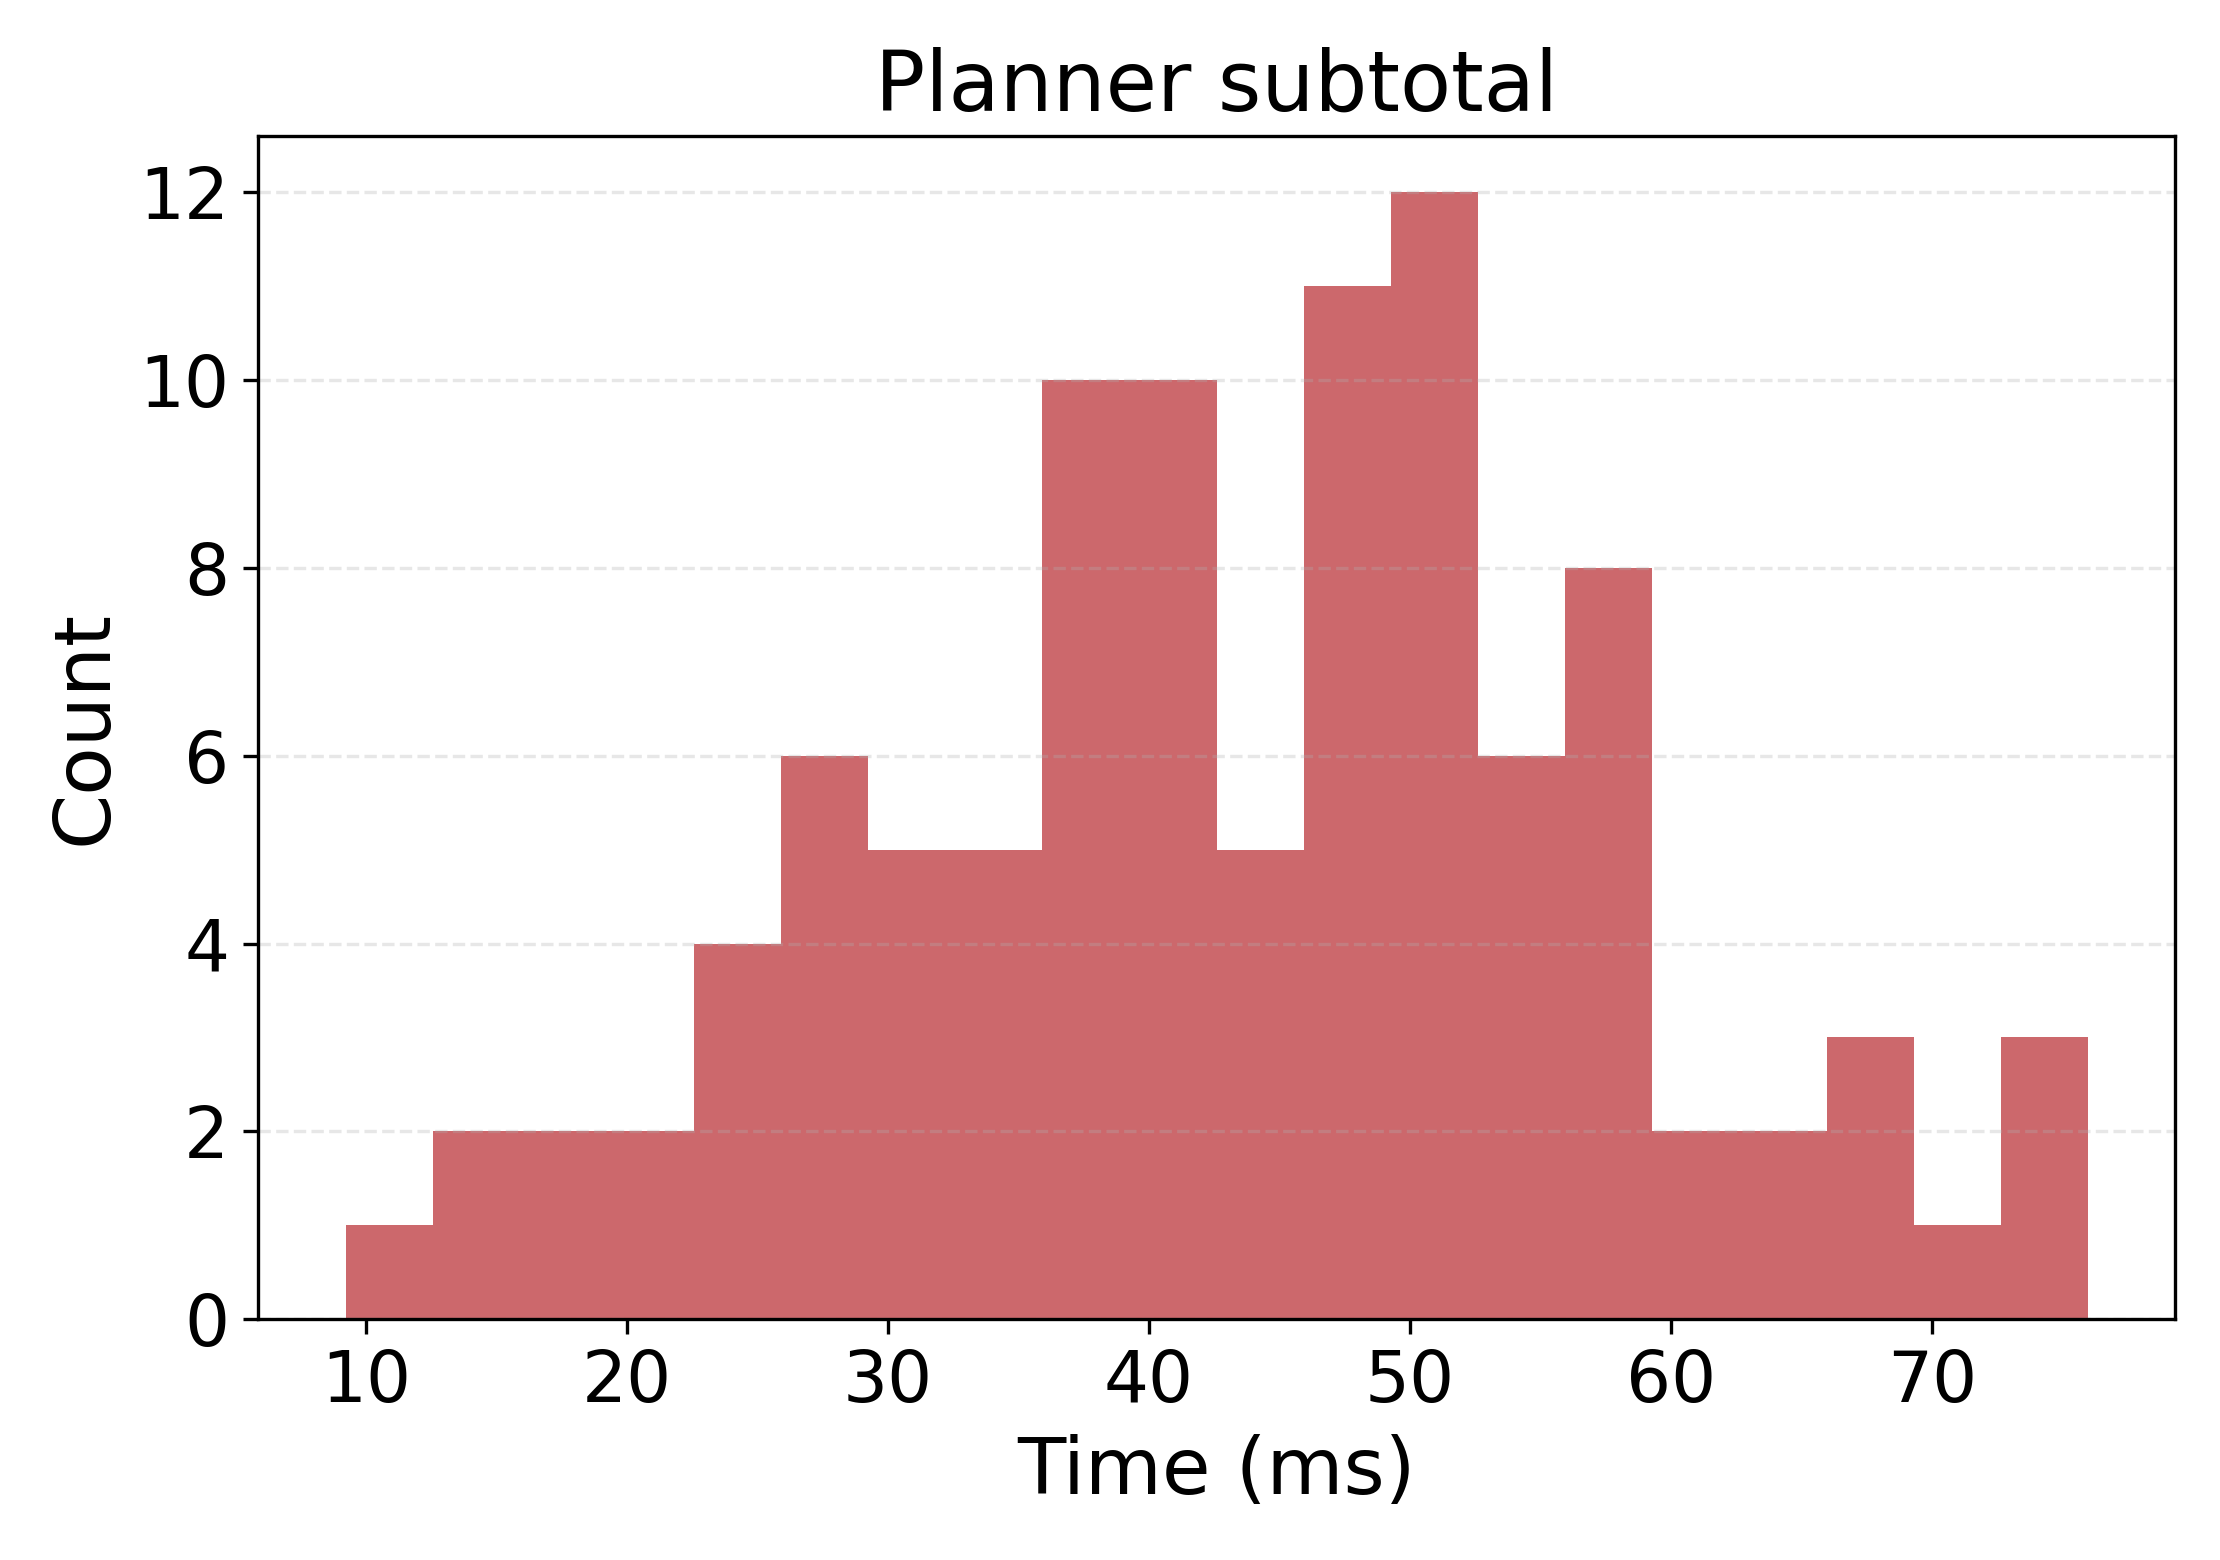
\includegraphics[width=0.46\textwidth]{figures/dist_planner_ms.png}}
  \hfill
  \subfloat[CFMS invocation + generation]{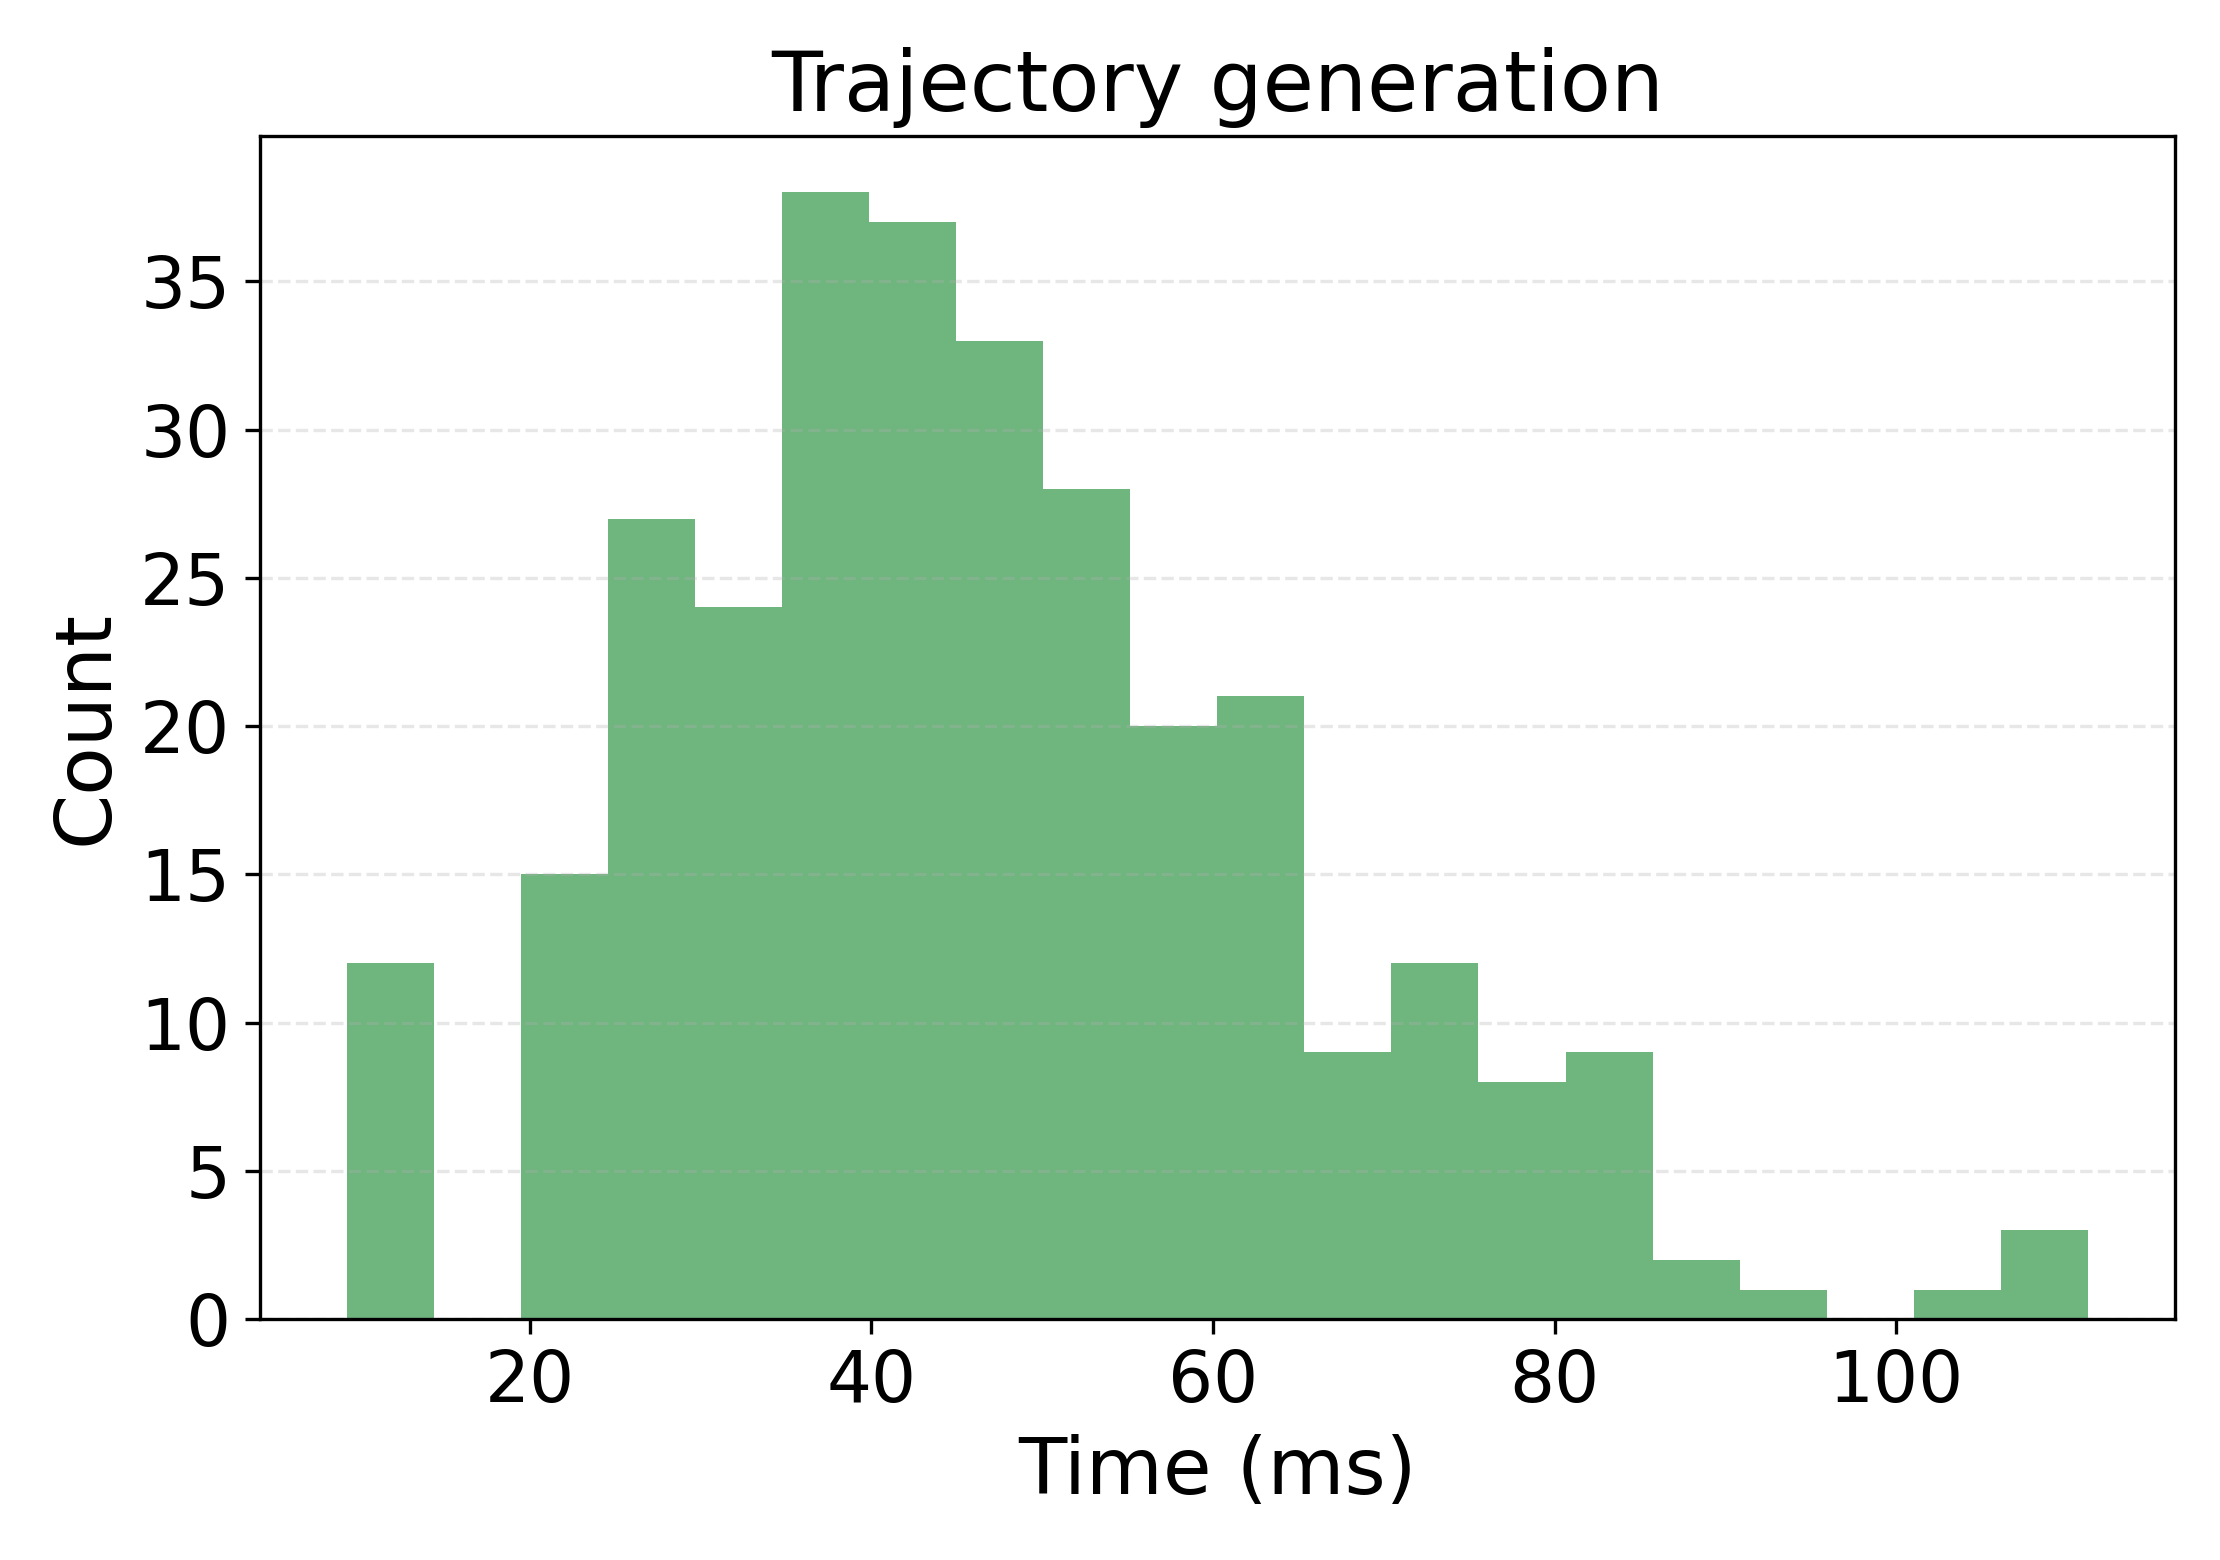
\includegraphics[width=0.46\textwidth]{figures/dist_traj_generator_ms.png}}\\
  \subfloat[Waypoint synthesis]{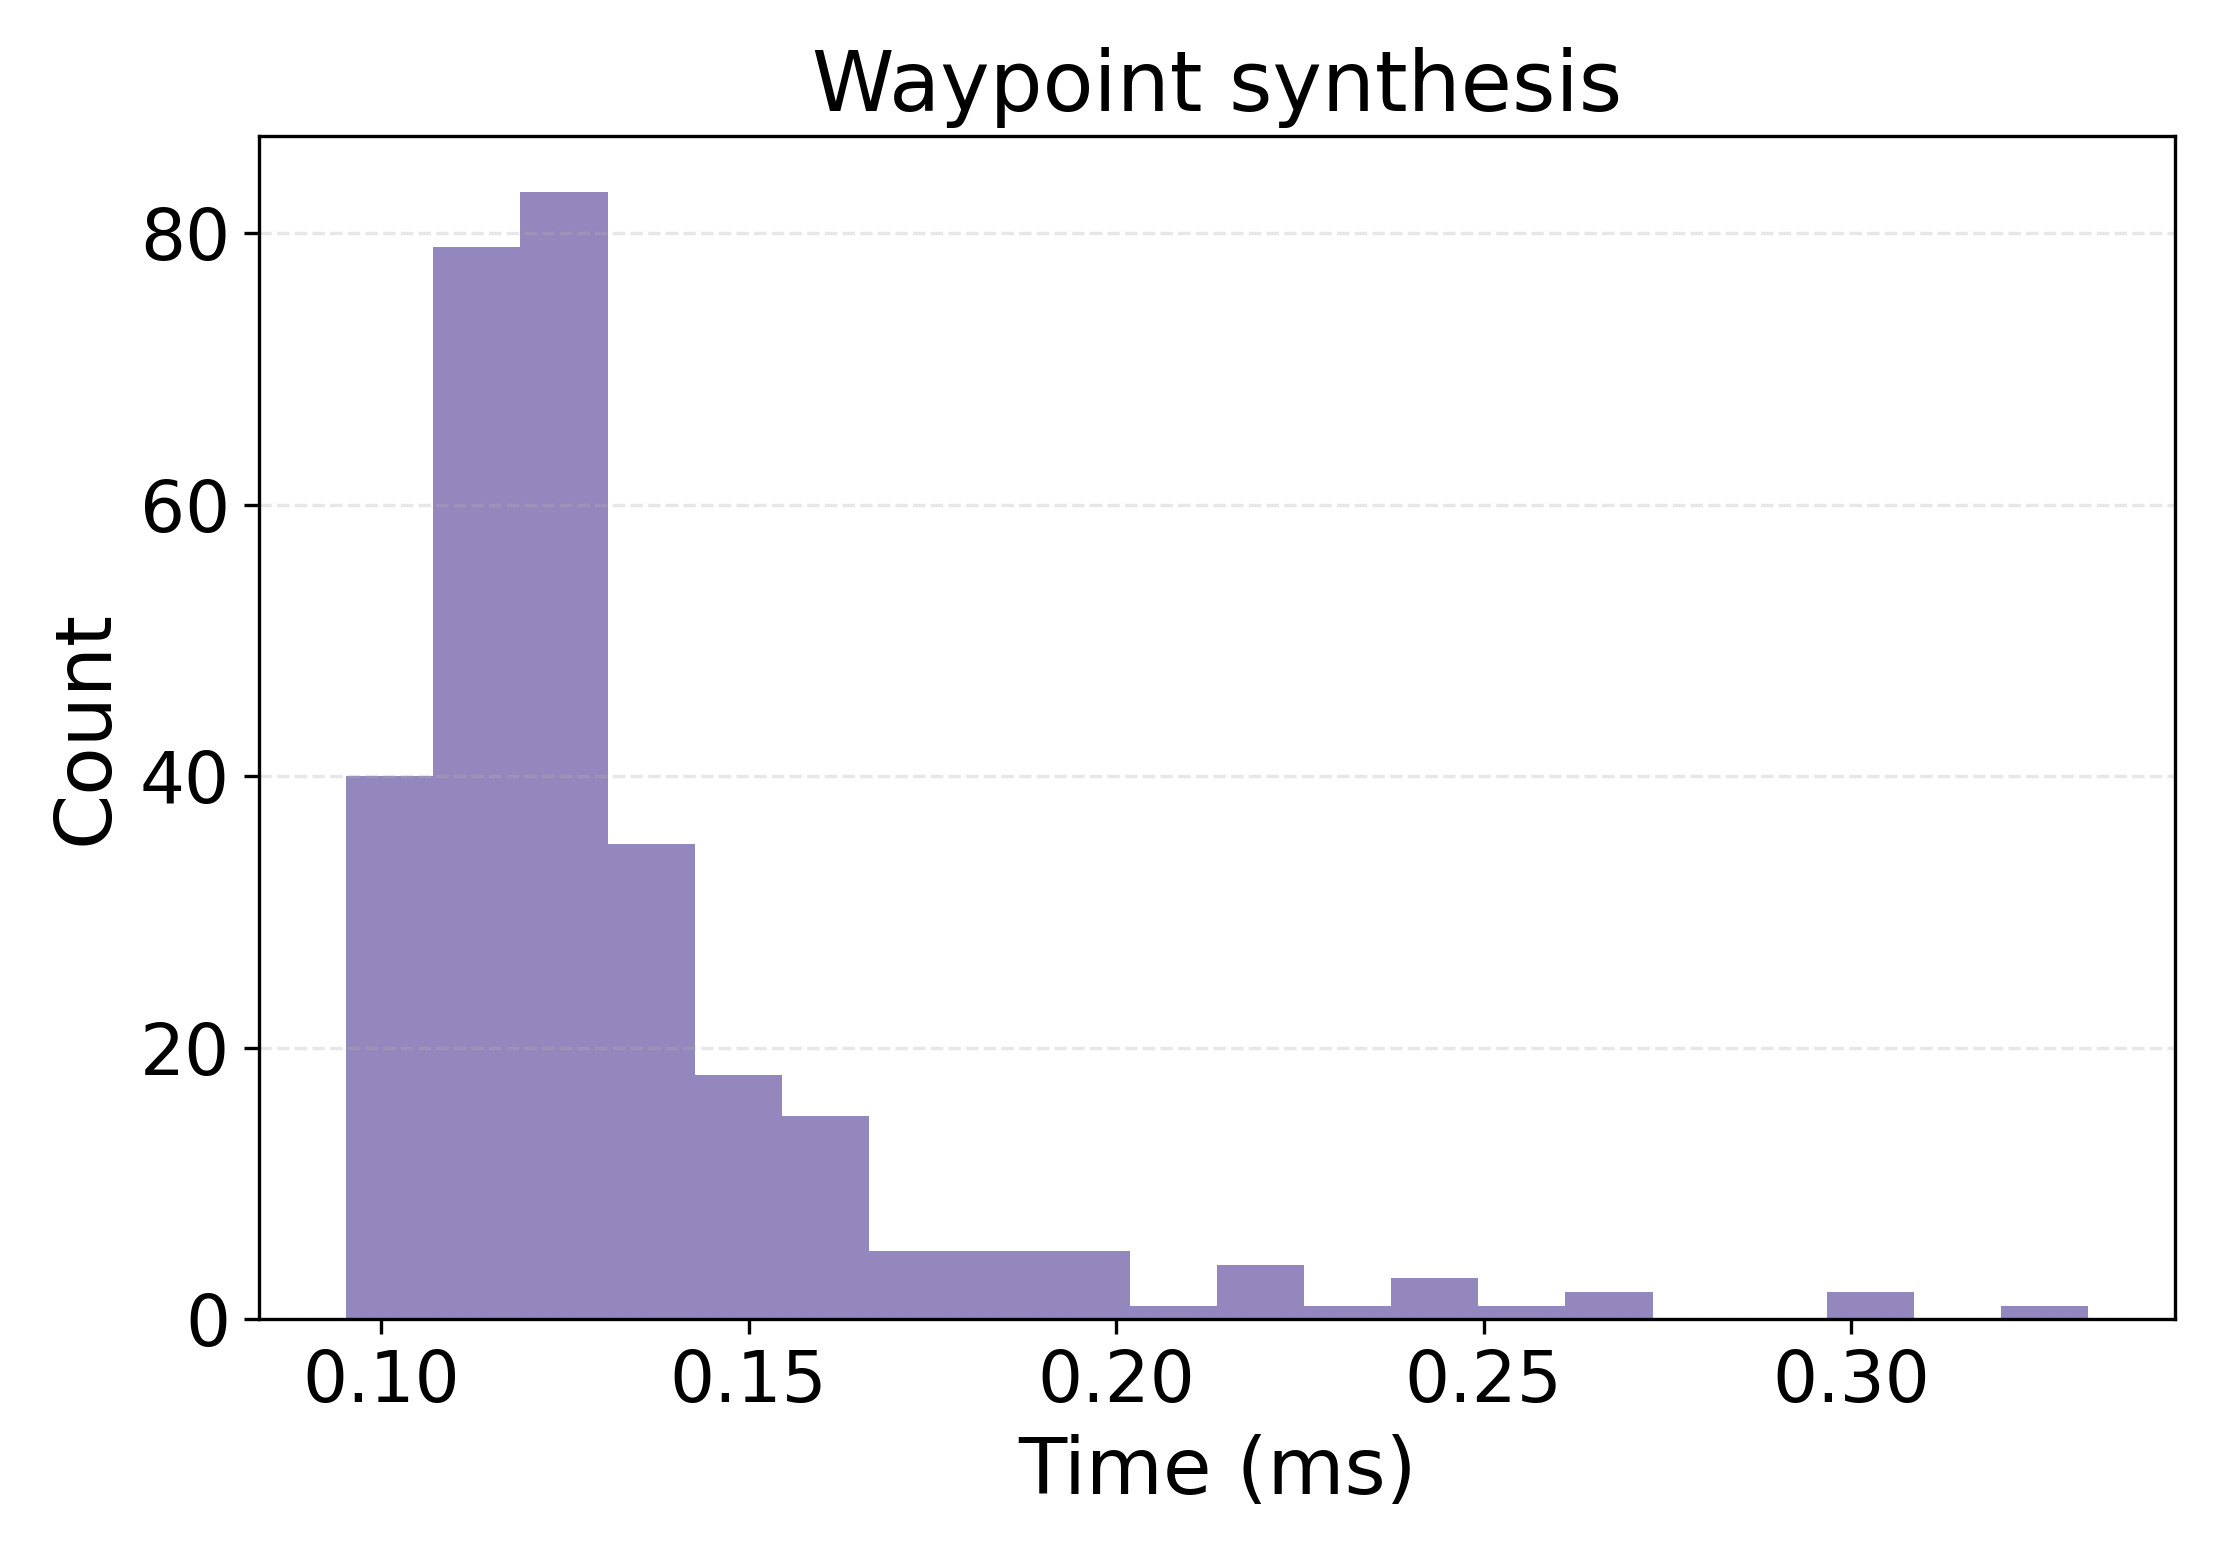
\includegraphics[width=0.46\textwidth]{figures/dist_waypoints_ms.png}}
  \hfill
  \subfloat[A* path search]{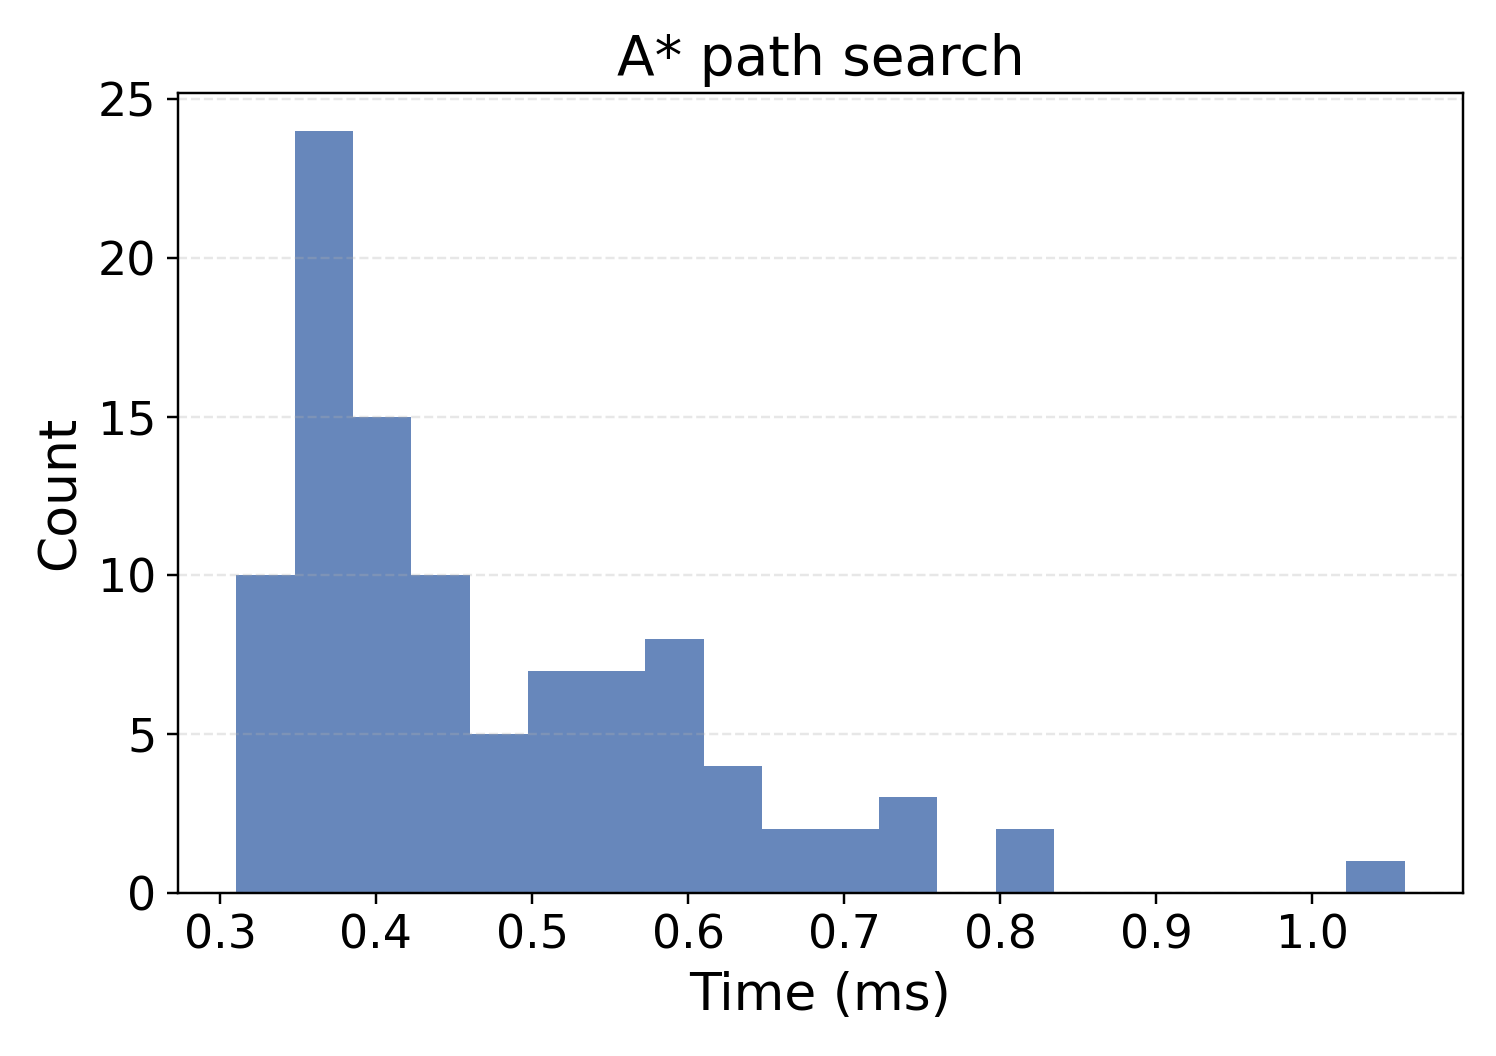
\includegraphics[width=0.46\textwidth]{figures/dist_astar_ms.png}}
  \caption{Planner-stage runtime distributions over the \paObs{} timing observations of the sequential benchmark (\paPairs{} OD pairs measured \paReps{} times each).}
  \label{fig:planner_scalability_hist}
\end{figure}

\subsection{Conflict-Resolution-Enabled Evaluation}
\label{sec:conflict_resolution_results}

A second sequential batch of \cfRequests{} requests was run with conflict checking and lateral re-routing enabled, using the detector configuration and closest-approach reporting of Section~\ref{sec:conflict_detection}. Every accepted trajectory was kept as a peer for the later requests. For each new request, the Planning Service first generated a candidate trajectory and then sent it to the Deconfliction Service. Any conflicts were mapped to route edges and resolved by lateral re-routing (Section~\ref{sec:conflict_resolution}), until no conflict was detected, no route remained, mapping stalled, or the limit of five attempts was reached. In the following, \emph{conflict-free} denotes this outcome status---no conflict detected under the sampled predicate of Equation~(\ref{eq:conflict_predicate})---and not a proof of continuous-time separation (Section~\ref{sec:conflict_detection}).

\paragraph{Traffic-density scenarios.}
Table~\ref{tab:conflict_density} repeats the same request sequence with the scheduling window reduced from the full day to 60, 30 and 15 minutes. All four runs use the same OD sequence, order and schedule-time seed, so they compare one traffic sample with itself under a shorter time window; they are not samples of a traffic population. In this run, the number of detected conflicts increases as the window is shortened, and the dense runs show outcomes that the full-day run does not have: requests that reached the retry limit, and requests with no route left, where re-routing runs out of alternatives because all remaining routes are blocked or the origin has no free edge anymore. Mapping stalls did not happen in any run. Since only requests without a detected conflict become peers, the rejected requests also make the peer set smaller: over the full day all \cfRequests{} plans are kept, but only \cfSixtyRetained{}, \cfThirtyRetained{} and \cfDenseRetainedMin{} in the 60, 30 and 15 minute windows. The conflicts in the dense runs are therefore counted against a peer set that is itself thinned out by the density, which slows down the growth of both conflicts and detection cost. For the evaluated request sequence, the share of requests with a first-check conflict among the requests with at least one overlapping peer increased from \cfConflictRate{}\% (full day) to \cfFifteenRate{}\% (15 minutes); these shares are not estimates of general conflict probabilities. Even in the densest window, far more pairs overlap in time than conflicts are detected, because overlap in time only decides which pairs are checked. The median detour of resolved requests stays moderate (between \cfDenseDetourMedianMin{} and \cfDenseDetourMedianMax{} in the dense windows), and the longest accepted detour has a ratio of \cfDenseDetourMax{}. Requests that were abandoned at the retry limit had even longer routes---up to \cfDenseDetourAbandonedMax{} times their first shortest route in the 15-minute window---but these routes were never accepted, so we report them separately. The largest ratios happen on short first routes, where one blocked edge forces a detour around a large part of the network: the \cfDenseDetourAbandonedMax{} case starts from a \SI{\cfDenseDetourAbandonedMaxInitialKm}{km} direct connection.

\begin{table}[H]
  \centering
  \caption{Traffic-density scenarios: identical OD sequence and seeds, schedule-time window compressed from 24 h to 15 min. Overlapping pairs are candidate--peer pairs with intersecting flight windows; the percentage row gives, among requests with at least one overlapping peer, the fraction that had an initial conflict; it is a request-level quantity, not a ratio of conflicting to overlapping pairs, and describes this single fixed-seed run rather than a population estimate. Every run additionally contains one empty-peer-set request. ``Retained as peers'' counts the requests that ended with no detected conflict and therefore became peers for later requests; retry-limit and no-route requests are rejected and excluded.}
  \label{tab:conflict_density}
  % Table generated by tools/make_conflict_tables.py; do not edit by hand.
  \begin{tabular}{lrrrr}
  \toprule
  & Full day & 60 min & 30 min & 15 min \\
  \midrule
  Conflict-free first check & 96 & 55 & 44 & 30 \\
  Resolved by re-routing & 3 & 20 & 24 & 30 \\
  Retry limit (5 attempts) & 0 & 8 & 12 & 15 \\
  No route left & 0 & 16 & 19 & 24 \\
  Mapping stalls & 0 & 0 & 0 & 0 \\
  Retained as peers at end of run & 100 & 76 & 69 & 61 \\
  Requests with initial conflict & 3 & 44 & 55 & 69 \\
  Temporally overlapping pairs & 118 & 1376 & 2105 & 2414 \\
  Conflict rate given overlap & 5.1\% & 54.3\% & 69.6\% & 93.2\% \\
  Blocked directed edges & 4 & 173 & 266 & 369 \\
  \bottomrule
\end{tabular}

\end{table}

\paragraph{Full-day baseline.}
All \cfRequests{} requests ended with an accepted, locally deconflicted plan: \cfClear{} were conflict-free at the first check, one---the first request---had no peers to check against, and \cfResolved{} were solved by lateral re-routing. Over the full day, temporal overlap between pairs was rare: only \cfOverlapPairs{} of \cfComparisons{} candidate--peer pairs overlapped. Per request it was more common, and \cfWithOverlap{} of the \cfWithPeers{} requests with at least one peer had at least one peer overlapping in time. Detected conflicts were still rare in this run: only \cfConflicted{} of these \cfWithOverlap{} requests (\cfConflictRate{}\%) had a conflict at the first check, so even when two flights were airborne at the same time, they were usually sufficiently separated. The \cfResolved{} resolved requests needed \cfAttemptList{} planning attempts, blocked \cfBlockedEdges{} directed edges in total, and had detour ratios of \cfDetourList{} compared with their first shortest route. No request reached the retry limit, and there were no mapping stalls or routing errors. With only \cfResolved{} conflicts, this run demonstrates the expected operation of the loop under the evaluated conditions, but it is not a statistical estimate of resolution performance. Figure~\ref{fig:conflict_resolution_eval} shows the outcomes and attempt counts, and Table~\ref{tab:conflict_resolution_cases} lists every conflict case.

\begin{figure}[!htbp]
  \centering
  \subfloat[Final request outcomes]{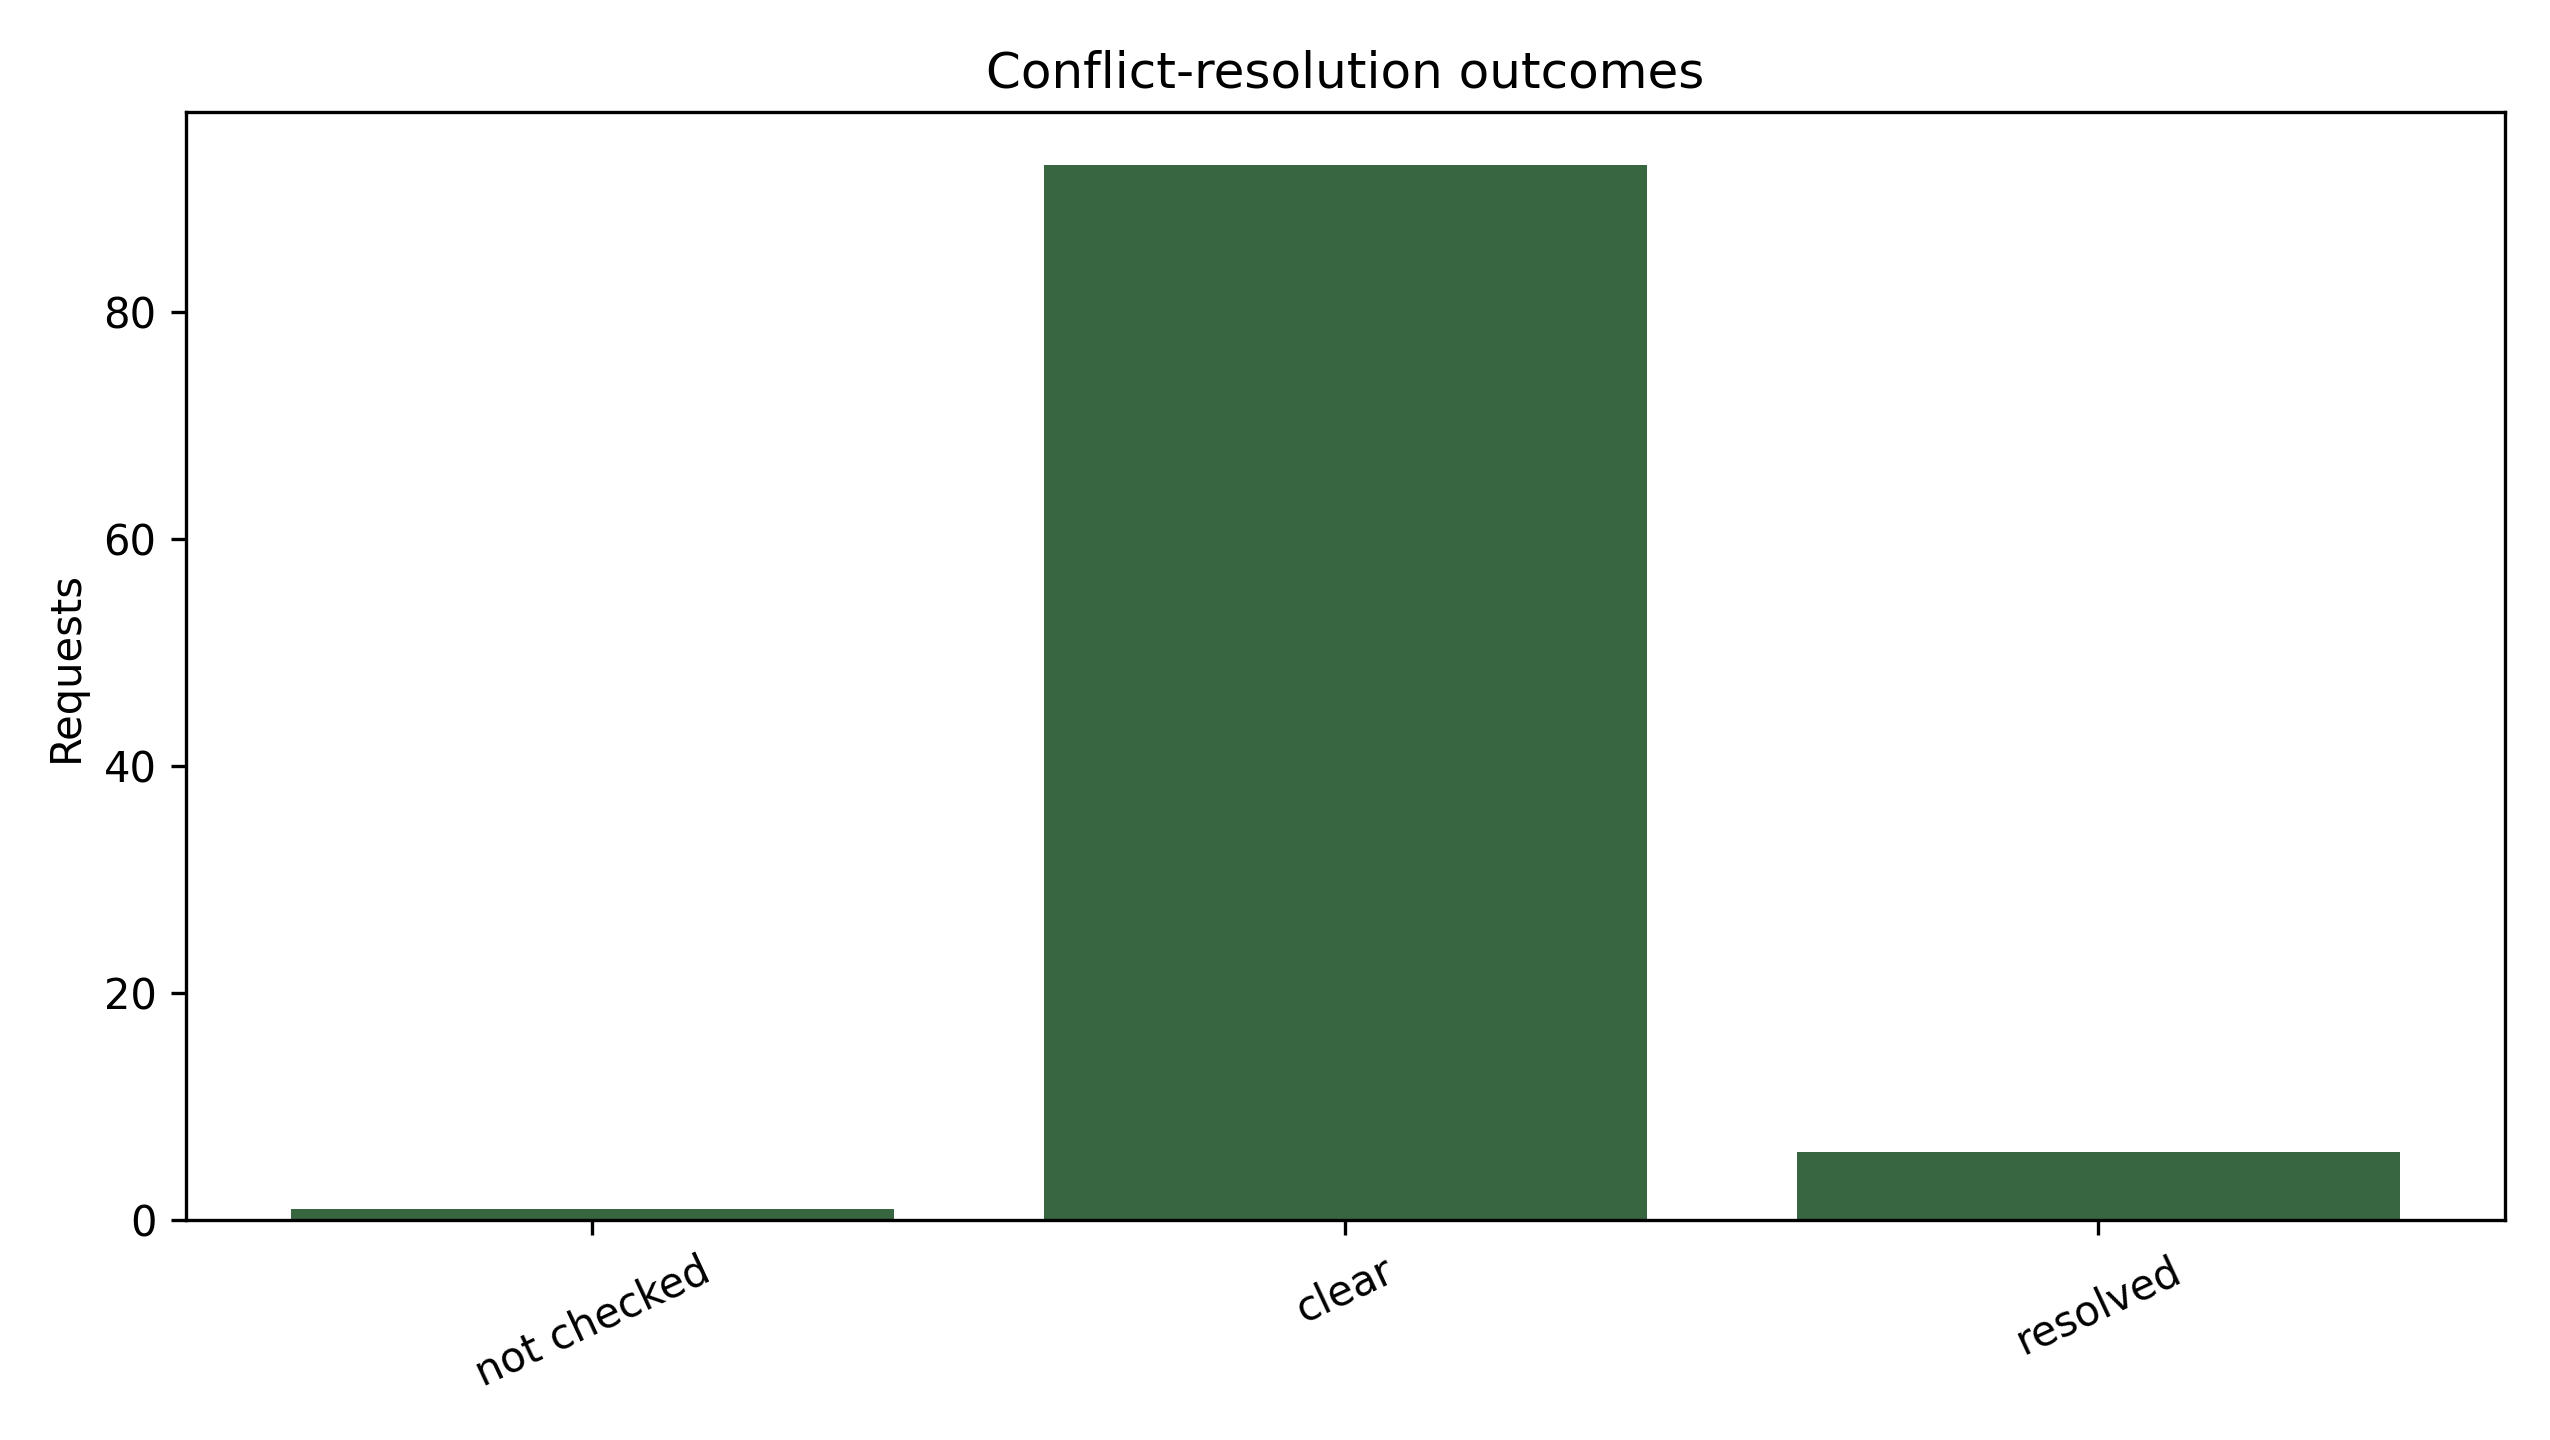
\includegraphics[width=0.48\textwidth]{figures/conflict_resolution_status_counts.png}}
  \hfill
  \subfloat[Planning attempts for checked requests]{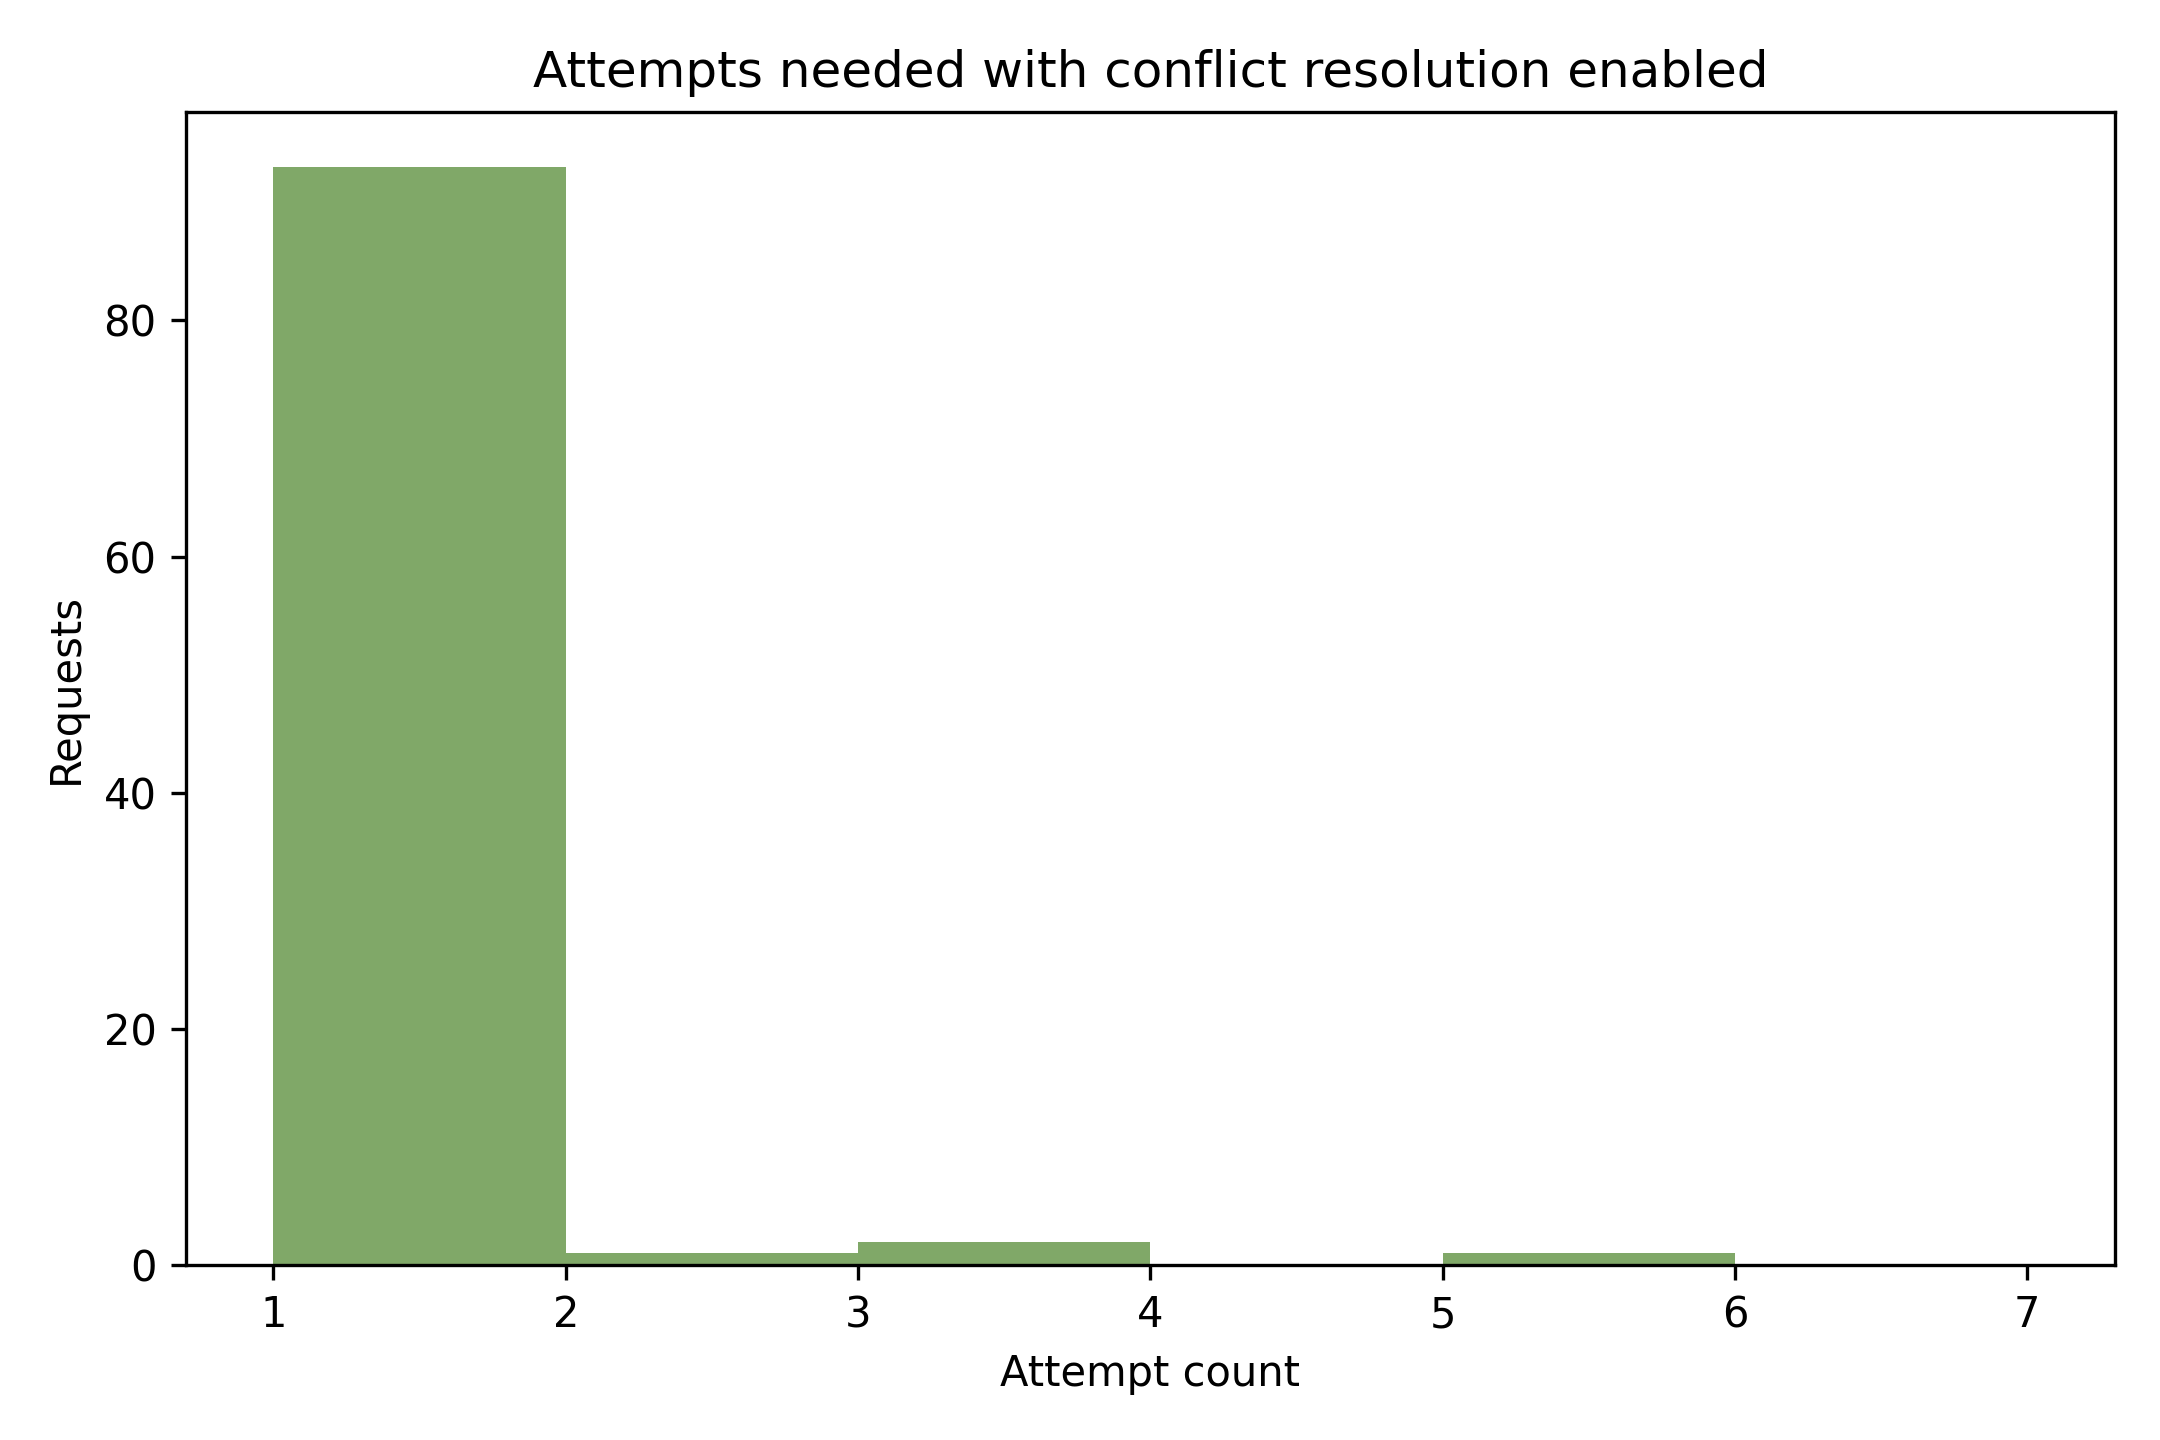
\includegraphics[width=0.48\textwidth]{figures/conflict_resolution_attempts.png}}
  \caption{Conflict-resolution-enabled evaluation over \cfRequests{} sequential full-day trajectory requests. Left: final request outcomes; ``Empty peer set'' is the first request, which has no peer to check against. Right: planning attempts per checked request; the axis spans the configured range of one to five attempts, and bar heights are request counts.}
  \label{fig:conflict_resolution_eval}
\end{figure}

\begin{table}[H]
  \centering
  \small
  \caption{All conflict cases of the full-day baseline run. Attempts = planning attempts; blocked edges are request-local directed removals; encounter types are classified from the blocked edge and the conflicting peer's route direction; peers = number of peer trajectories available at request time; detour = final over initial route distance; plan and detect are the summed per-attempt planner and conflict-detection times; end-to-end is the client-observed request time; status ``Resolved'' means resolved by lateral re-routing. Initial and final routes are contained in the archived per-request results.}
  \label{tab:conflict_resolution_cases}
  \footnotesize
  \setlength{\tabcolsep}{3.5pt}
  % Table generated by tools/make_conflict_tables.py from the evaluation outputs
  % in plots/conflict_resolution/. That tool also corrects the generator's
  % peer_set_size, which counts an accepted candidate as one of its own peers.
  % Do not edit by hand; rerun the tool instead.
  \begin{tabular}{@{}p{1.35cm}cp{2.15cm}p{1.75cm}ccrrrp{1.3cm}@{}}
  \toprule
  OD pair & Att. & Blocked edges & Encounter & Peers & Detour & \makecell{Plan\\(ms)} & \makecell{Detect\\(ms)} & \makecell{E2E\\(ms)} & Status \\
  \midrule
  \texttt{HMLE--BLAN} & 2 & VOLK\(\to\)BLAN & head-on & 31 & 1.5682 & 221.72 & 1806.72 & 2058.03 & Resolved by re-routing \\
  \texttt{HARB--HSEN} & 3 & HCTY\(\to\)HSEN; WILH\(\to\)HCTY & node-crossing & 45 & 1.0603 & 221.67 & 4599.58 & 4848.91 & Resolved by re-routing \\
  \texttt{BLAN--WNTH} & 2 & BLAN\(\to\)VOLK & same-direction & 72 & 1.7908 & 245.49 & 4501.12 & 4792.99 & Resolved by re-routing \\
  \bottomrule
\end{tabular}

\end{table}

\paragraph{End-to-end latency decomposition.}
Figure~\ref{fig:conflict_latency_decomposition} splits the total request time seen by the client into planning (including storing the results), the conflict-checking service call, and residual request overhead, separately for requests that were conflict-free at the first check and for resolved requests. Conflict-free requests take \cfClearClientMs{}~ms on average, of which only \cfClearPlanMs{}~ms is planning and \cfClearOverheadMs{}~ms is residual request overhead; the other \cfClearDetectMs{}~ms is the single conflict-detection call. Resolved requests take \cfResolvedClientMs{}~ms on average, with \cfResolvedPlanMs{}~ms planning, \cfResolvedDetectMs{}~ms detection summed over all attempts, and \cfResolvedOverheadMs{}~ms overhead. The detection-stage measurement covers the current stateless workflow: as described in Section~\ref{sec:conflict_detection}, every check reloads the candidate and all peer trajectories---up to 99 at the end of the run, each with around one thousand samples---and rebuilds the detector state from scratch. The measured block covers the service call, trajectory fetching, detector-state construction and NDMap execution together. Their individual contributions were not instrumented, so neither the intrinsic NDMap query time nor the communication cost can be isolated. Residual overhead is client-observed time minus the summed planning and detection blocks; it includes request handling, serialization and conflict-to-edge mapping outside those blocks, not only transport. With this workflow, a conflict-checked request takes more than ten times longer than the planner-stage subtotal of Section~\ref{sec:planner_scalability}, and the detection stage is the main measured cost here. The growth with the peer set can be seen inside the run. We compare the first and the last quarter of the requests that were conflict-free at the first check, in the order they arrived; both groups make exactly one detection call, so their means can be compared directly. Detection time increases from \cfClearDetectFirstMs{}~ms with \cfClearDetectFirstPeersLo{}--\cfClearDetectFirstPeersHi{} peers to \cfClearDetectLastMs{}~ms with \cfClearDetectLastPeersLo{}--\cfClearDetectLastPeersHi{} peers, about seven times more (\(n = \cfClearDetectFirstN{}\) requests per group). The run means therefore average over a cost that is still growing at the end of the sequence.

\begin{figure}[!htbp]
  \centering
  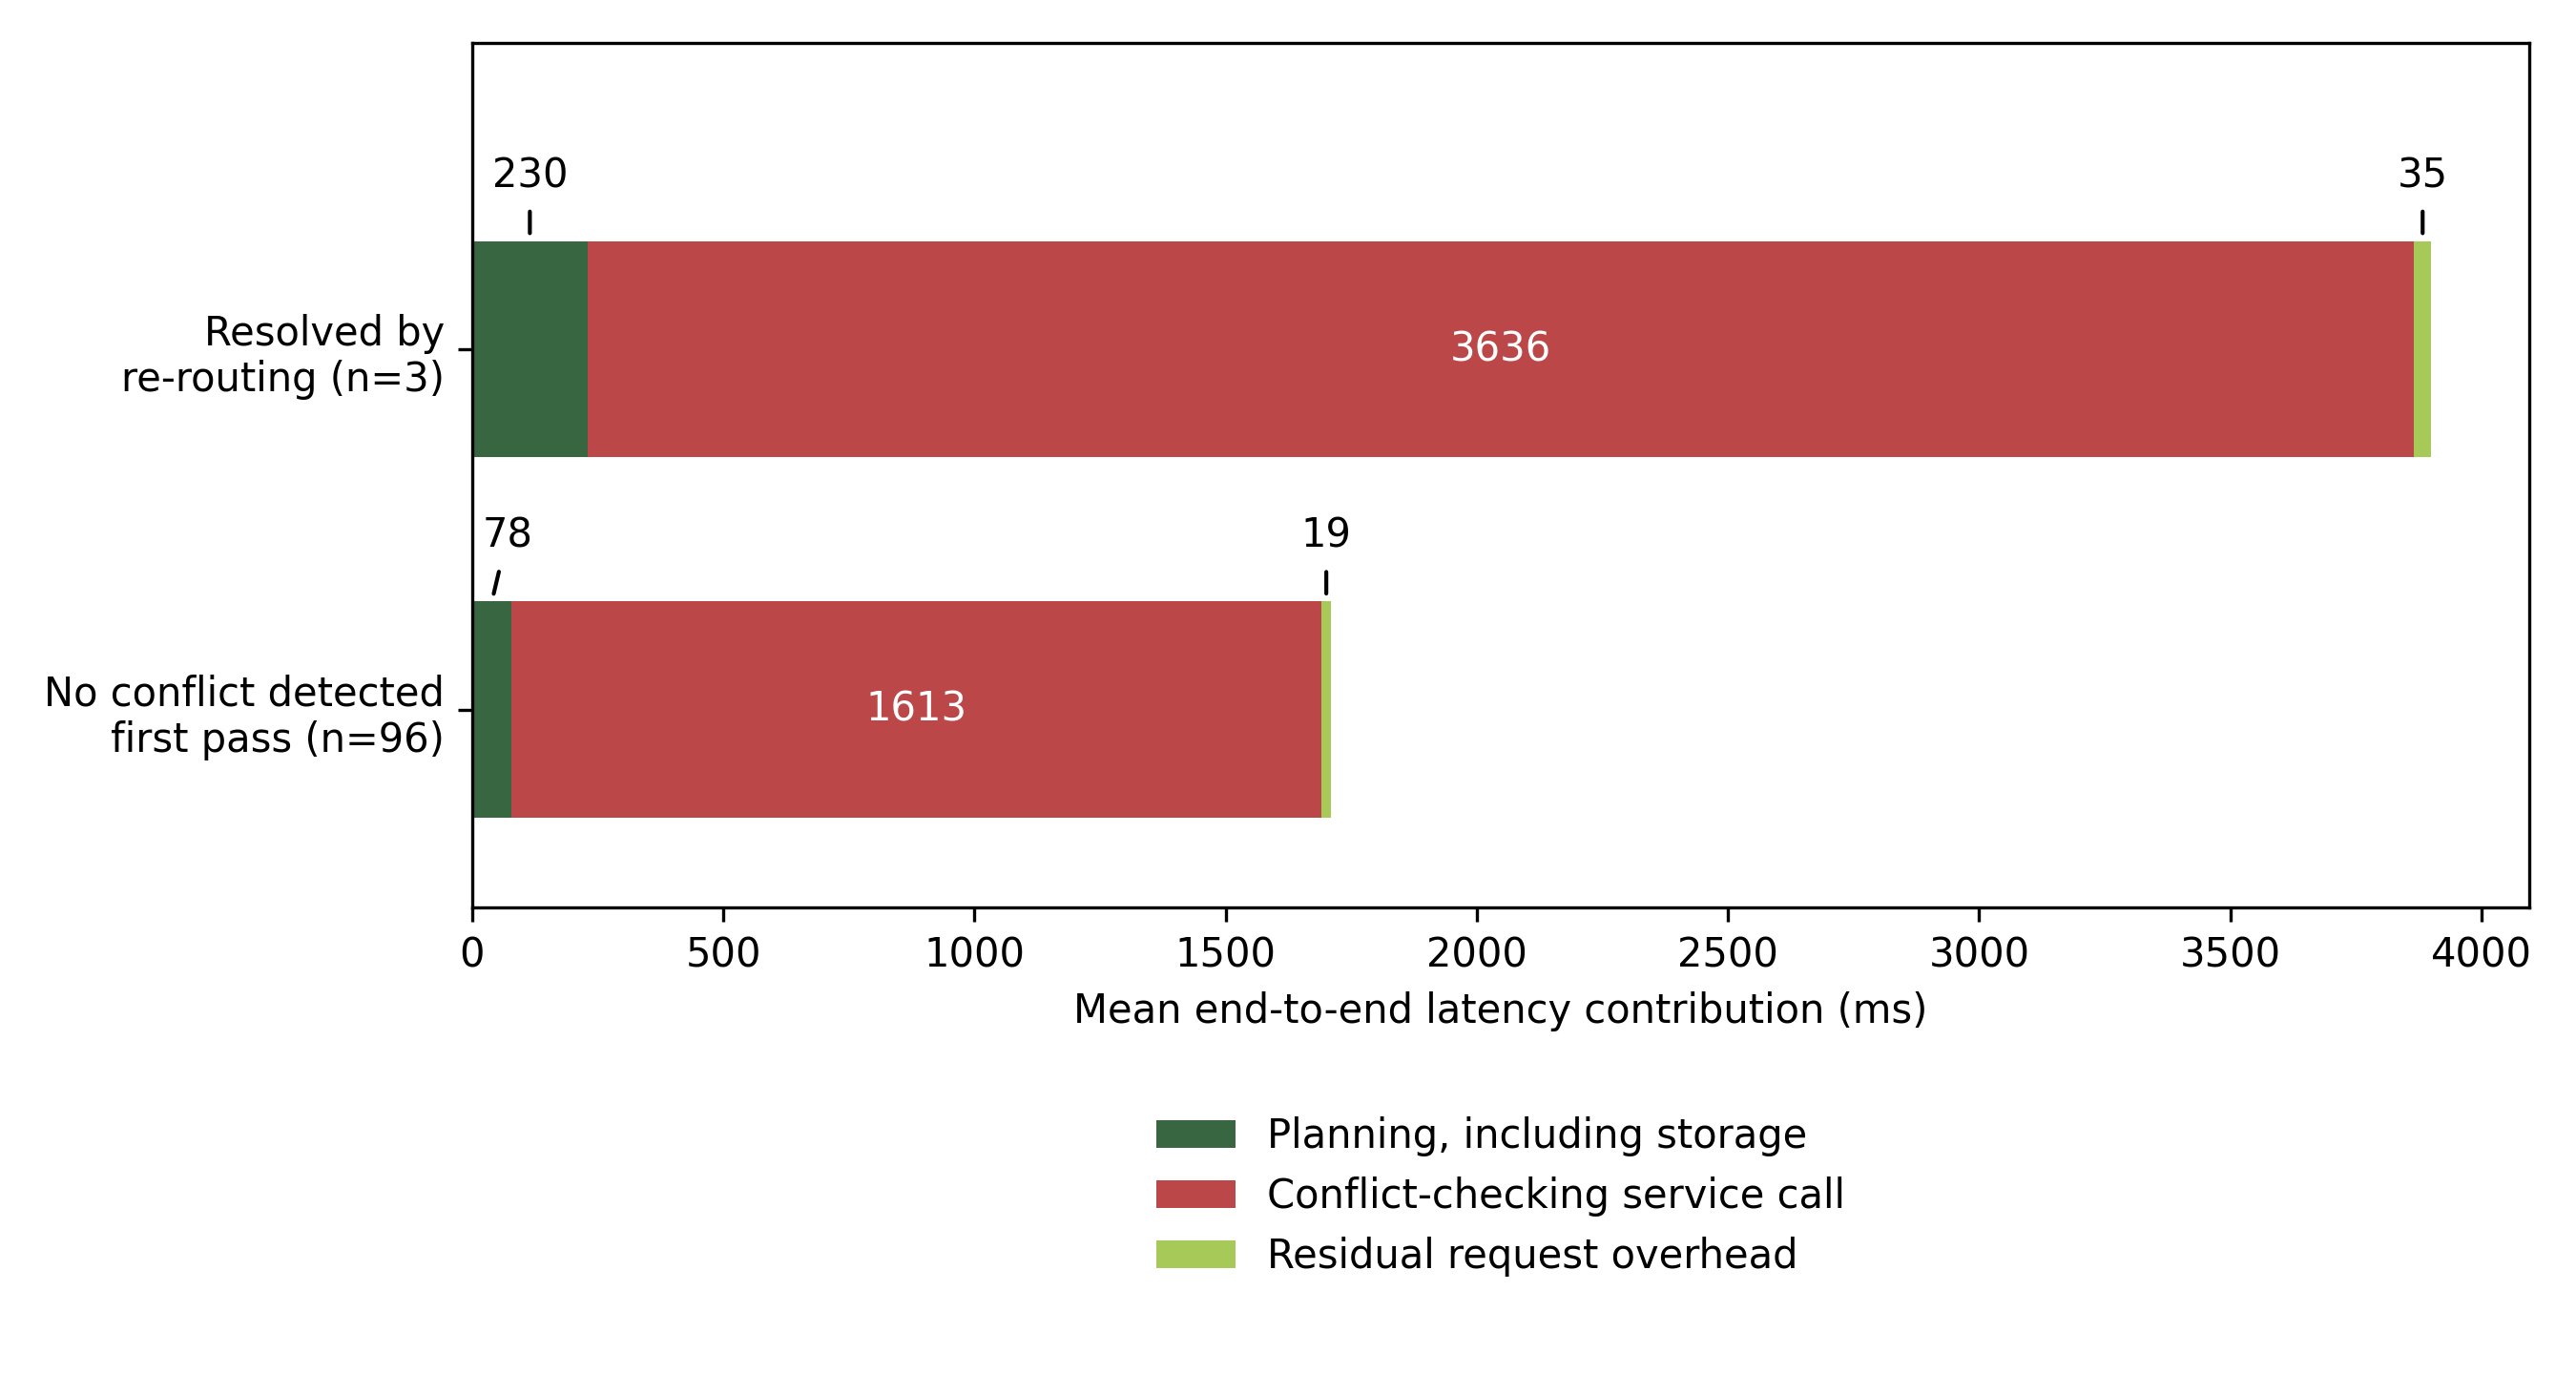
\includegraphics[width=0.85\textwidth]{figures/conflict_resolution_latency_decomposition.png}
  \caption{Mean end-to-end latency decomposition for the full-day run, split into planning including artifact persistence (dark green), conflict detection including peer trajectory fetch and detector-state rebuild (red), and residual request overhead (light green). The residual includes all work outside the two timed blocks and is not an isolated network measurement. Top: requests resolved by re-routing (sums over all attempts, \(n=\cfResolved{}\)); bottom: requests with no conflict detected at the first check (\(n=\cfClear{}\)). Segment labels give the mean contribution in milliseconds.}
  \label{fig:conflict_latency_decomposition}
\end{figure}

\paragraph{Deterministic encounter cases.}
Table~\ref{tab:deterministic_cases} separates the scripted assertions from the observed resolution statuses. Initial conflicts were detected in the head-on, following, crossing and merge setups. The head-on and crossing requests were resolved; the following and shared-destination requests exhausted the reduced graph. The crossing run also recorded a mapped conflict within \SI{556}{m} of the shared node, a diagnostic rather than an independent accuracy test of closest-approach reporting. The last check repeats the merge geometry and timing with a different candidate identifier, so the five checks represent four distinct setups. All scripted assertions passed, but most assert initial detection only. These observations demonstrate the loop's behavior on selected encounters, not completeness of lateral resolution. In particular, failure of the following case does not establish that all possible lateral routes would conflict. For the shared-destination setup, fixing both flights to the same pad and landing time preserves an endpoint incompatibility regardless of the lateral approach; the observed no-route status still results from the implemented edge-removal strategy.

\begin{table}[H]
  \centering
  \small
  \caption{Scripted encounter checks and observed outcomes. All five assertions passed; the fifth repeats the fourth setup. Initial conflicts are reported on the first check. A no-route status refers to the reduced graph after edge removals.}
  \label{tab:deterministic_cases}
  \begin{tabularx}{\textwidth}{lXlr}
    \toprule
    Case & Scripted assertion & Observed status & Initial conflicts \\
    \midrule
    Head-on, same route & initial conflict detected & resolved & 1 \\
    Following, \SI{15}{s} in trail & initial conflict detected & no route left & 3 \\
    Crossing at graph node & initial conflict detected & resolved & 1 \\
    Merge at shared destination & initial conflict detected & no route left & 2 \\
    Repeated shared-pad setup & non-resolution & no route left & 2 \\
    \bottomrule
  \end{tabularx}
\end{table}

\FloatBarrier
